\documentclass[a4paper,11pt]{article}
\usepackage[utf8]{inputenc}
\usepackage[T1]{fontenc}
\usepackage{geometry}
\geometry{
  top=2.5cm,
  bottom=1.5cm,
  left=2cm,
  right=2cm,
  footskip=.2cm
}
\usepackage{XCharter}
\usepackage{graphicx}
\usepackage[hidelinks]{hyperref}    
\usepackage{color}
\usepackage[document]{ragged2e}
% \pagestyle{empty}                   
\usepackage{enumitem}               
\usepackage{float}
\usepackage{titlesec}
\usepackage{wrapfig}
\usepackage{pdfpages}
\setlist[itemize]{itemsep=-2pt, leftmargin=12pt, topsep=7pt} 
\graphicspath{{../../lebenslauf/pictures/}}
 \setlength{\skip\footins}{1.5cm}
\definecolor{sections}{rgb}{0, 0.5, 0.2}
\definecolor{links}{rgb}{0, 0.5, 0.5}
\hypersetup{
    colorlinks=true,    
    urlcolor=links,      
    pdfborder={0 0 0}     
}
% gs -dBATCH -dNOPAUSE -sDEVICE=pdfwrite -dCompatibilityLevel=1.4  -dPDFSETTINGS=/printer -sOutputFile=Resume.pdf lebenslauf.pdf
\titleformat{\section}
  [runin]
  {\normalfont\bfseries}
  {\thesection}                    % <-- Nummer wieder aktiviert
  {0.5em}                          % kleiner Abstand zwischen Nummer und Text (statt 0pt)
  {}
  [.]

\titlespacing*{\section}
  {0pt}{3.25ex plus 1ex minus .2ex}{1em}   % same spacing values \section uses by default
 
\usepackage{titletoc}
\titlecontents{section}
  [0pt]                              % Einzug links
  {}                                 % oberhalb
  {\contentslabel{2em}}              % <-- mit Nummer: Label + Breite reservieren
  {}                                 % ohne Nummer (falls \section* o.ä.)
  {\titlerule*[1pc]{.}\contentspage} % Punkte + Seitenzahl

% Überschrift unterdrücken:
\renewcommand{\contentsname}{}

\begin{document}

\begin{titlepage}
	\thispagestyle{empty}
	\begin{flushright}
		\setlength{\fboxsep}{8pt}
		\begin{minipage}{0.4\textwidth}
			\raggedleft
			Fynn Gewiese\\
			Xaver Handel\\
			Timo Drüen\\
			Tobias Belm\\
			\today
		\end{minipage}
	\end{flushright}
	\vspace{2\baselineskip}
	% --- Main title block, centered ---
	\begin{center}
		\vspace*{5\baselineskip}
		{\textcolor{sections}{\Huge\bfseries Report\\}}
		\vspace{0.5\baselineskip}
		{\Large Projekt GateMate SS26\\}
		\vspace{0.3\baselineskip}
		{\large HM bei Prof.\ Dr.\ Felix Miller}
		\vspace{2\baselineskip}
		% \begin{figure}[H]
		% 	\centering
		% 	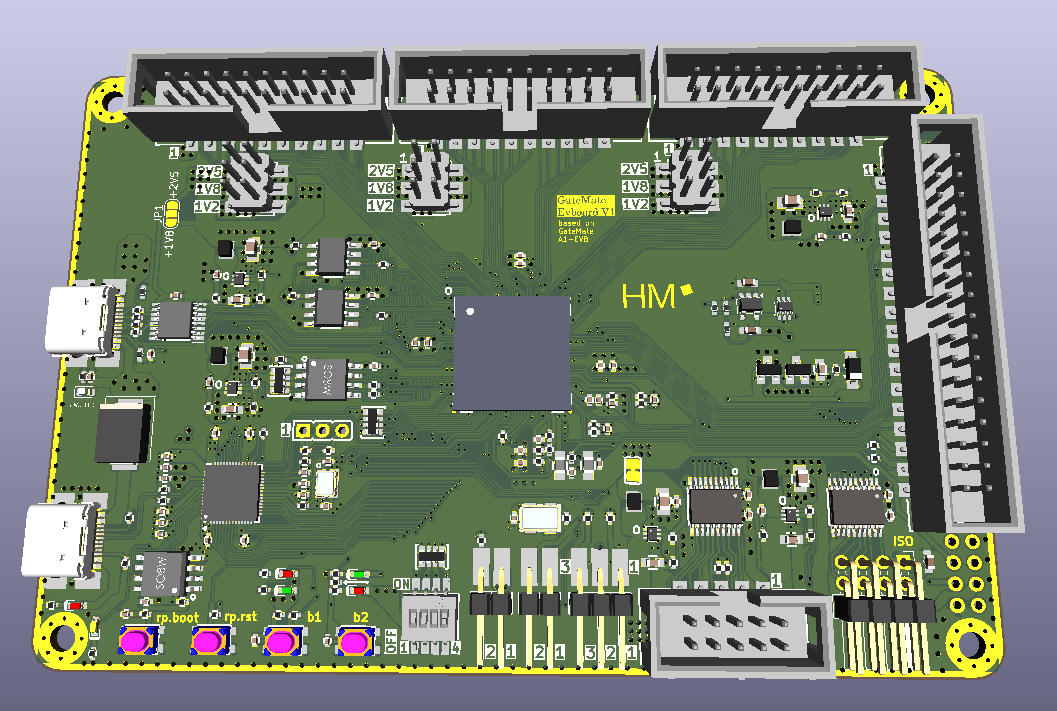
\includegraphics[width=0.9\textwidth]{assets/MillerV1.png}
		% 	\caption{PCB Render}
		% 	\label{fig:millerv1}
		% \end{figure}
	\end{center}
	\vfill
\end{titlepage}
\newpage
\pagenumbering{arabic}
\setcounter{page}{2}

\section{Abstract / Ziel des Projektes | Fynn}
Der GateMate-FPGA von Cologne Chip ist als europäischer FPGA von besonderem Interesse, da er eine Alternative zu den marktdominierenden Anbietern aus den USA und Asien darstellt\footnote{\url{https://colognechip.com/programmable-logic/gatemate/}}. Gerade im Hinblick auf technologische Souveränität und Unabhängigkeit von außereuropäischen Lieferketten gewinnt die Verfügbarkeit einer solchen, vollständig in Europa entwickelten FPGA-Plattform zunehmend an Bedeutung. Hinzu kommt, dass für den GateMate im Gegensatz zu vielen etablierten FPGA-Familien eine offene Toolchain existiert, wodurch sich die Architektur besonders gut für Lehre, Forschung und Open-Source-Projekte eignet. Olimex bietet mit dem GateMate-A1-EVB ein Evaluationsboard an, das vollständig als Open-Source-Hardware verfügbar ist\footnote{\url{https://www.olimex.com/Products/FPGA/GateMate/GateMateA1-EVB/open-source-hardware}}, sodass sämtliche Schaltpläne, Layouts und Bauteilinformationen frei zugänglich sind und als verlässliche Ausgangsbasis für eigene Entwicklungen dienen können. Dieses Board kann als Grundlage genommen werden werden, um darauf eine Smart Card zu realisieren, die sich sowohl als Master als auch als Slave betreiben lässt und damit flexibel in unterschiedlichen Anwendungsszenarien eingesetzt werden kann. Ziel war es dabei, ein System zu schaffen, das sich für Weiterentwicklungen und Anpassungen eignet, ohne von proprietärer Hardware oder geschlossenen Toolchains abhängig zu sein. Dafür werden im Wesentlichen drei Komponenten benötigt: ein ISO-Interface zur Kommunikation nach dem ISO/IEC-7816-Standard, eine USB-Schnittstelle zur Anbindung an einen Host-Rechner sowie ein IBEX-RISC-V-Prozessor\footnote{\url{https://github.com/lowrisc/ibex}}, der als frei verfügbarer, open-source Prozessorkern die zentrale Steuerungs- und Verarbeitungslogik der Smart Card übernimmt.

\begin{figure}[H]
	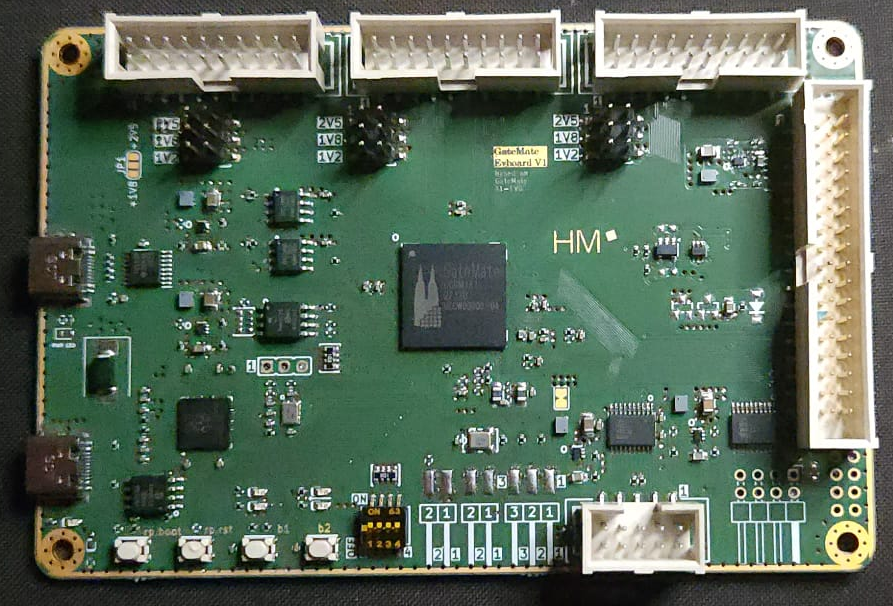
\includegraphics[width=0.99\textwidth]{assets/pcb_pretty.png}
	\caption{PCB nach dem Löten}
	\label{fig:pcb_pretty}
\end{figure}

\newpage
{\normalfont\bfseries    Inhaltsverzeichnis}\\
\tableofcontents

\newpage

\section{Arbeitsaufteilung | Fynn}
Im Rahmen des Projekts habe ich die Rolle des Group Leaders und Organisators übernommen.
Dazu gehörte das Aufsetzen der GitHub-Struktur als zentrale Plattform für die Zusammenarbeit,
sowie die Erarbeitung der Requirements,
auf deren Basis das Projekt weiterentwickelt wurde.
Darauf aufbauend habe ich die anfallenden Teilaufgaben aufgestellt und den einzelnen Teammitgliedern zugewiesen.
Zusätzlich habe ich die Entwicklung des USB-Transceivers supervisiert und die zuständigen Teammitglieder fachlich angeleitet.
Neben Anpassungen des OLIMEX Evaluationboards wurde von mir auch das ISO/IEC 7816 Interface designed.
Zuletzt habe ich am Löten des Projektes teilgenommen, die Platine in fast funktionsfähingen Zustand gebracht
und mit Xaver and der fehlenden Clockgeneration gearbeitet.
\vspace{\baselineskip}

\textbf{Xaver:}\\
Verantwortlich für den gesamten Software- und FPGA-Ressourcen-Teil des Projekts. Xaver hat den Ibex RISC-V Core erfolgreich auf die Architektur des GateMate-FPGAs portiert, die SystemVerilog-Module (insbesondere RAM, Bussystem und Register File) an die Hardware-Limitierungen angepasst und die notwendige Toolchain (Yosys, nextpnr, DirtyJTAG) eingerichtet. Außerdem hat er die UART-Schnittstelle implementiert, Workarounds für das auf dem FPGA fehlende Clock-Gating entwickelt und den Ablauf zur C-Code-Generierung für den RISC-V Core realisiert.

\vspace{\baselineskip}
\textbf{Timo:}\\
Übernahm das BOM-Management (Sourcing-Strategie, Distributor-Konsolidierung über DigiKey) und war maßgeblich für die Component Substitution (Finden passender Ersatzbauteile für nicht lieferbare Komponenten) zuständig. Zudem definierte Timo die Pin-Constraints für den USB-PHY, erstellte den iterativen Bringup- und Testplan und war zusammen mit Fynn intensiv an der manuellen Bestückung und Verlötung des Prototyps (Reflow-Verfahren) beteiligt.

\vspace{\baselineskip}
\textbf{Tobias (Tobi):}\\
Fokussierte sich auf das Hardware-Design der Kommunikationsschnittstellen. Tobi entwickelte das Schaltungskonzept für den USB-2.0-PHY (TUSB1106), definierte die USB-C-Power-Topologie (inkl. Schutzdioden) und erarbeitete die Spezifikationen für das ISO/IEC-7816-Interface. Zur späteren Verifikation programmierte er ein umfangreiches VHDL-Testmodul, das die USB-Serial-Interface-Engine (SIE) nachbildet und elementare USB-Transaktionen (Token-Responder) ermöglicht.


\newpage
\section{PCB Aufarbeitung | Fynn}
Ein wesentlicher Teil meiner Arbeit bestand in der Überarbeitung der Platine.
Die ursprünglich unstrukturierte Schematic habe ich in thematisch klar abgegrenzte Blöcke restrukturiert, wodurch die Übersichtlichkeit und Wartbarkeit deutlich verbessert wurde.
Darüber hinaus habe ich die Platine optisch aufgewertet, unter anderem durch das Einfügen des HM-Logos und einheitlicher Beschriftungen.
Um die Komplexität zu reduzieren, habe ich zudem ein Debloating der Platine durchgeführt und nicht benötigte Elemente entfernt.

% \begin{figure}[H]
% 	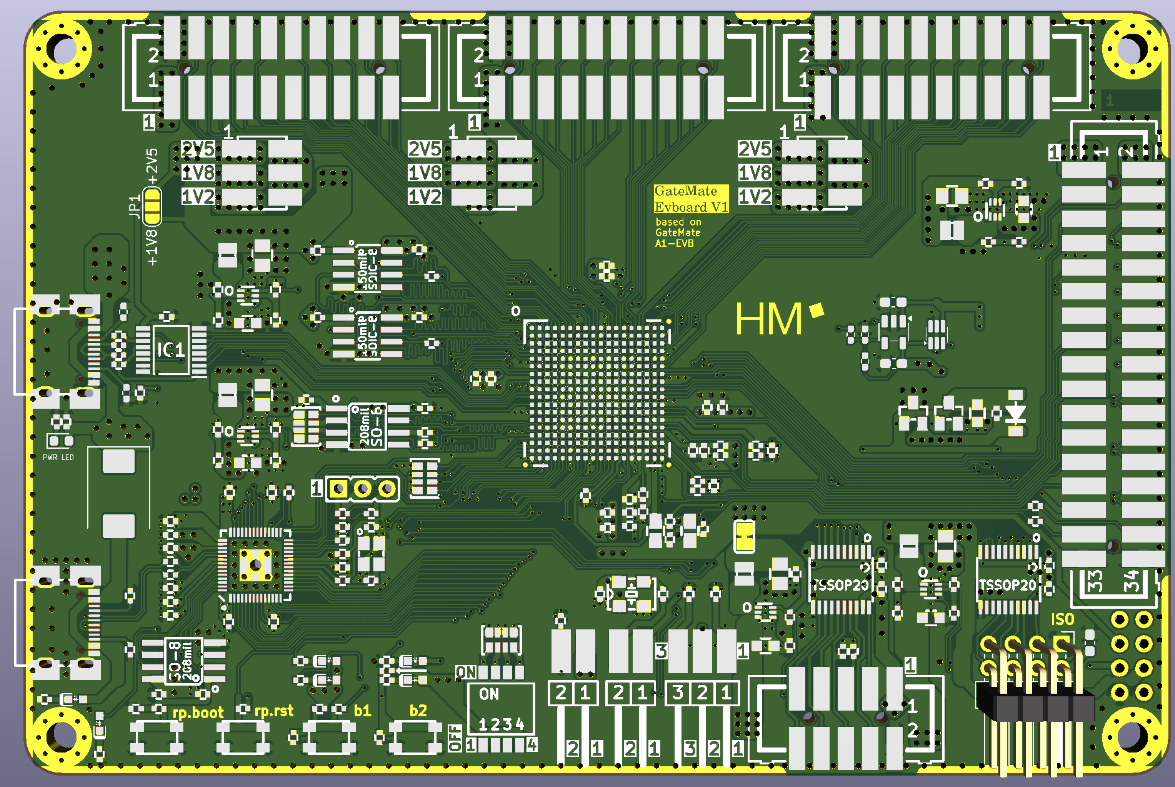
\includegraphics[width=0.8\textwidth]{assets/render_no_comp.png}
% 	\caption{3D render ohne Komponenten}
% 	\label{fig:render_no_comp}
% \end{figure}

Ein weiterer wichtiger Aspekt der Überarbeitung war die Sicherstellung einer kontrollierten Impedanz für die USB- und SRAM-Leitungen,
um Signalintegrität  zu gewährleisten und Reflexionen sowie Übersprechen zu minimieren.
Im Anschluss habe ich den Design Rule Check (DRC) durchgeführt und die daraus resultierenden notwendigen Änderungen umgesetzt.
Abschließend habe ich die Recherche geeigneter Hersteller übernommen und mich dabei bewusst für AISLER als lokalen Anbieter entschieden,
und die Bestellung der Platine veranlasst.

% \begin{figure}[H]
% 	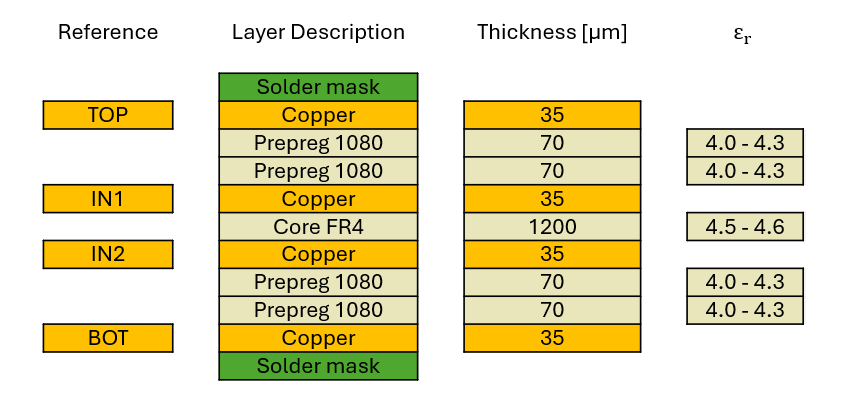
\includegraphics[width=0.8\textwidth]{assets/stackup.png}
% 	\caption{Verwendeter 4 Lagen PCB Stackup von AISLER}
% 	\label{fig:stackup}
% \end{figure}

\section{ISO/IEC 7816 Interface | Fynn}
Für die Kommunikation nach dem ISO/IEC-7816-Standard habe ich ein Interface entworfen,
das flexibel sowohl im Master- als auch im Slave-Betrieb eingesetzt werden kann.
Dieser duale Ansatz ermöglicht eine breitere Einsatzfähigkeit der Platine,
da je nach Anwendungsfall zwischen beiden Betriebsmodi gewechselt werden kann.

\begin{figure}[H]
	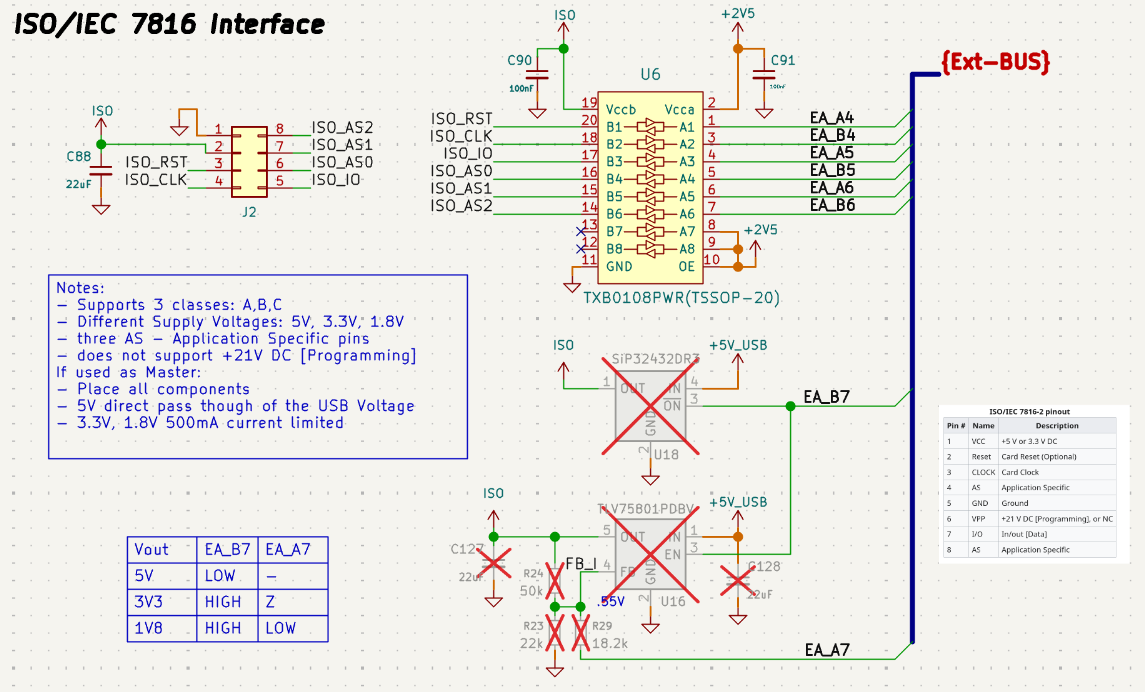
\includegraphics[width=0.8\textwidth]{assets/interface.png}
	\caption{ISO/IEC 7816 Interface Schematic}
\end{figure}

Ein zentrales Element ist der TXB0108-Levelshifter,
der den GPIO-Logikpegel des FPGA in den passenden Ausgangs-Logikpegel konvertiert.
Die Ausgangsspannung wird dabei entweder vom angeschlossenen Master bereitgestellt,
oder – falls der FPGA selbst als Master fungiert – wahlweise über einen Schalter (für 5V) oder einen LDO erzeugt.
Der LDO ist einstellbar (adjustable) und besitzt ein Feedback-Netzwerk aus Widerständen.
Der FPGA kann einen dieser Widerstände erden,
um die Ausgangsspannung zwischen 3.3V und 1.8V umzuschalten.

% \begin{figure}[H]
% 	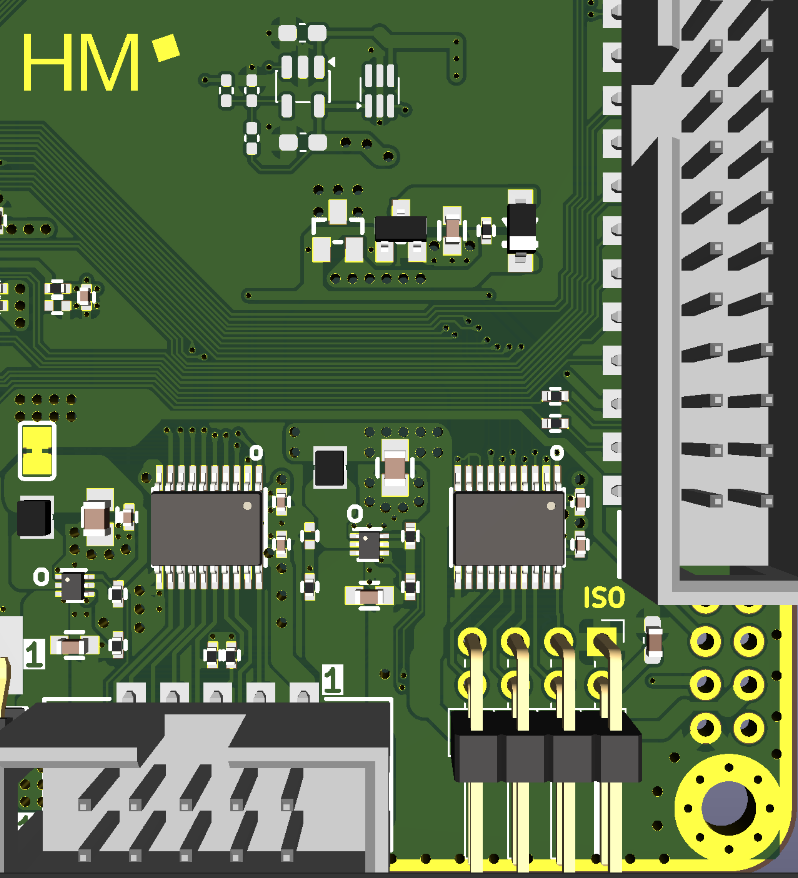
\includegraphics[width=0.5\textwidth]{assets/renderISO.png}
% 	\caption{ISO/IEC 7816 Interface Sektion auf der Platine}
% 	\label{fig:millerv1}
% \end{figure}

Das ISO/IEC-7816-Interface ist auf der Platine als Arduino-Header umgesetzt
und befindet sich als doppelte Stiftleiste unten rechts.
Direkt darüber ist der Levelshifter platziert.
Oben rechts, neben dem HM-Logo, befinden sich der LDO sowie der Switch zur Spannungsversorgung.
\newpage

\section{Problem der fehlenden Clock | Fynn \& Xaver}
Bei der Inbetriebnahme des FPGA-Boards zeigte sich, dass der SX5M10.000B10F20TNN 10 MHz XO Crystal Oscillator in der Stückliste fehlte und dem FPGA somit keine Taktquelle zur Verfügung stand.
Um die Ursache einzugrenzen, wurde das Problem parallel von zwei Seiten angegangen:
Fynn kümmerte sich um die Hardware, während Xaver die Funktionsfähigkeit auf Softwareebene überprüfte.
Xaver erstellte dazu Bitfiles für eine blinkende LED sowie sich ändernde Pins.
Mit unterschiedlichen Clock Quellen und Frequenzen.
Zusätzlich wurde ein Binary getestet, das die LED lediglich statisch auf High oder Low setzt und dementsprechend auch ohne funktionierenden Takt hätte laufen müssen –
da dieser Test ebenfalls fehlschlug, liegt die Vermutung nahe, dass neben der fehlenden Clock noch ein weiteres, bisher nicht identifiziertes Problem vorliegt.

\begin{wrapfigure}{l}{0.5\textwidth}
	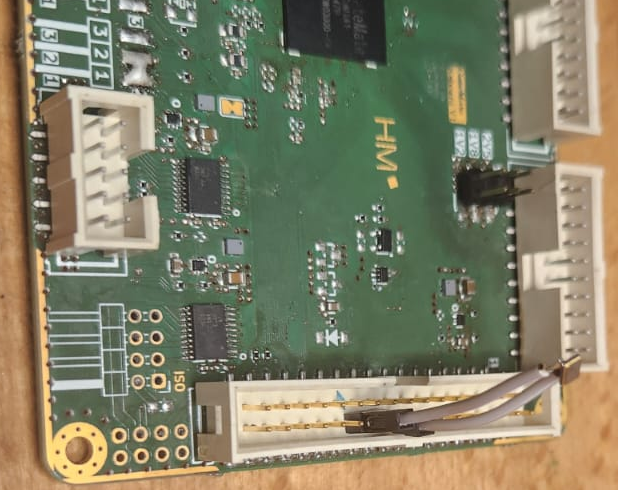
\includegraphics[width=0.5\textwidth]{assets/floating_crystal.png}
	\caption{FPGA mit eingestecktem Quarz}
	\label{fig:floating_crystal}
\end{wrapfigure}
Auf Hardwareseite wurden mehrere Ansätze verfolgt, um dem FPGA dennoch einen Takt zur Verfügung zu stellen.
Da die Serial-Clock-Pins nach außen geroutet sind, wurde zunächst versucht, einen gewöhnlichen Quarz direkt einzustecken (siehe Abbildung \ref{fig:floating_crystal}).
Dieser Versuch verlief ohne Erfolg.


% \begin{figure}[H]
% 	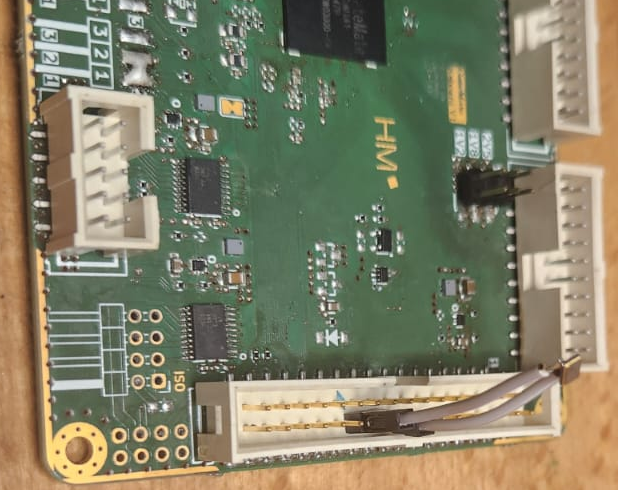
\includegraphics[width=0.5\textwidth]{assets/floating_crystal.png}
% 	\caption{FPGA mit eingestecktem Quarz}
% 	\label{fig:floating_crystal}
% \end{figure}

Im nächsten Schritt wurde ausgenutzt, dass Clock 1 und Clock 2 über den Debugger zugänglich sind.
Der Debugger wurde entsprechend umprogrammiert, um darüber ein Taktsignal anzulegen – auch dieser Ansatz führte nicht zum gewünschten Ergebnis.
Da Clock 0 und Clock 3 extern eingespeist werden können, wurde schließlich versucht, ein Signal im Bereich von 100 kHz bis 100 MHz von außen anzulegen.
Auch hierbei konnte an keiner Stelle ein funktionierender Takt erzeugt werden, sodass das Problem der fehlenden Clock zum jetzigen Zeitpunkt weiterhin ungelöst bleibt.


\section{Verbesserungsvorschläge für spätere Iterationen | Fynn}
Aus den gesammelten Erfahrungen dieser Revision ergeben sich mehrere Punkte, die in einer nächsten Iteration der Platine berücksichtigt werden sollten.
So sollten die beiden USB-C-5V-LEDs, die aktuell separat ausgeführt sind, zu einer einzigen LED zusammengefasst werden, um unnötige Redundanz zu vermeiden.
Ebenso sollte die Stückliste insgesamt verkleinert werden, wobei insbesondere die Anzahl der verwendeten Kondensatoren reduziert werden kann.
10nF Condensatoren im gleichen Package wie 2.2uF Kondensatoren sind fast ein direktes Downgrade,
v.a. da weder Inrush-Current noch der minimal höhere Preis hier eine Rolle spielen.
Für die Spannungsversorgung bietet sich der Einsatz eines Power-ICs mit mehreren integrierten Buck-Convertern an,
anstatt die einzelnen Spannungsebenen wie bisher getrennt zu realisieren.

Darüber hinaus stellte sich während der Inbetriebnahme heraus, dass der verbaute RP2040-Flash-Speicher nicht funktionierte;
ein Ersatz durch einen entsprechenden Baustein von Winbond hingegen funktionierte einwandfrei und sollte für zukünftige Revisionen als Referenz dienen.
Aus noch unerforschten Gründen ging auch der Winbond Ersatz nach einer Weile kaputt und musste getauscht werden.
Symptopme hierfür ist, das der RP2040 auch nach dem Flashen den Bootmodus nicht verlässt.

Zuletzt wäre eine LED hilfreich,
die die funktionstüchtigkeit der letzten Stromversorgung anzeigt.
Das ist nämlich ein starkes Symptom dafür,
das die anderen Stromversorgungen auch funktionieren,
da diese kaskadieren.
\newpage

\section{Serial to USB transceiver | Tobias}

\textbf{Recherche und Konzept}
\begin{itemize}
	\item Einarbeitung in den USB-2.0-PHY TUSB1106 von Texas Instruments.
	\item Einarbeitung in den ISO/IEC-7816-Standard für Smart-Card-Schnittstellen.
	\item Definition separater Power-Domains für den USB-PHY und das ISO/IEC-7816-Interface.
\end{itemize}

\textbf{USB-C-Power-Topologie}

Eine direkte Verbindung der VBUS-Pins beider USB-C-Ports hätte die jeweiligen 5-V-Schienen kurzgeschlossen beziehungsweise ungewollte Rückströme ermöglicht. Deshalb wurde Port~1 über Vias direkt mit \texttt{+5V\_USB} verbunden, während Port~2 durch eine Schottky-Diode vom Typ B340 (3~A, 40~V) entkoppelt ist. Dadurch werden die Power-Domains voneinander getrennt und Port~2 zusätzlich gegen Verpolung geschützt. Die berechnete VBUS-Spannung am TUSB1106 liegt trotz des Spannungsabfalls an der Diode komfortabel innerhalb der USB-2.0-Spezifikation. Eine Power-LED D2 mit einem 2,2-k$\Omega$-Vorwiderstand R35 an \texttt{+5V\_USB} dient als visuelle Betriebsanzeige.

% Abbildung: USB-C-Power-Topologie (Schottky-Diode B340) -- Datei fehlt aktuell
% \begin{figure}[H]
% 	\centering
% 	\includegraphics[width=0.8\textwidth]{assets/usb_c_power.png}
% 	\caption{USB-C-Power-Topologie mit Schottky-Diode B340}
% 	\label{fig:usb_c_power}
% \end{figure}

\textbf{Schematic des USB-PHY}
\begin{itemize}
	\item USB-C-Port~2 verwendet alle vier VBUS-Pins zur Erhöhung der Stromtragfähigkeit. CC1 und CC2 sind jeweils mit einem 5,1-k$\Omega$-Pull-down für die Device-Rolle beschaltet.
	\item Das USB-2.0-Differential-Pair ist für eine differentielle Impedanz von 90~$\Omega$ ausgelegt. Ergänzt wurden 33-$\Omega$-Serienterminierungen und ein 1,5-k$\Omega$-Pull-up zur Full-Speed-Erkennung.
	\item Der integrierte 5-V-zu-3,3-V-Regler des TUSB1106 wird über \texttt{VREG(3.3)} genutzt.
	\item Über den Jumper JP1 kann die I/O-Versorgung (VCC(I/O)) des TUSB1106 zwischen 1,8~V für den GateMate und alternativ 2,5~V gewählt werden. Das VBUS-Sensing erfolgt über VP und VM.
	\item Alle acht digitalen Signale des TUSB1106 (VM, VP, VPO, VMO, RCV, SUSPND, SPEED und OE) wurden gezielt über den Peri-BUS auf GateMate-FPGA-Pins wie \texttt{VGA\_Blue\_2} und \texttt{VGA\_Red\_2} geroutet.
\end{itemize}

\begin{figure}[H]
	\centering
	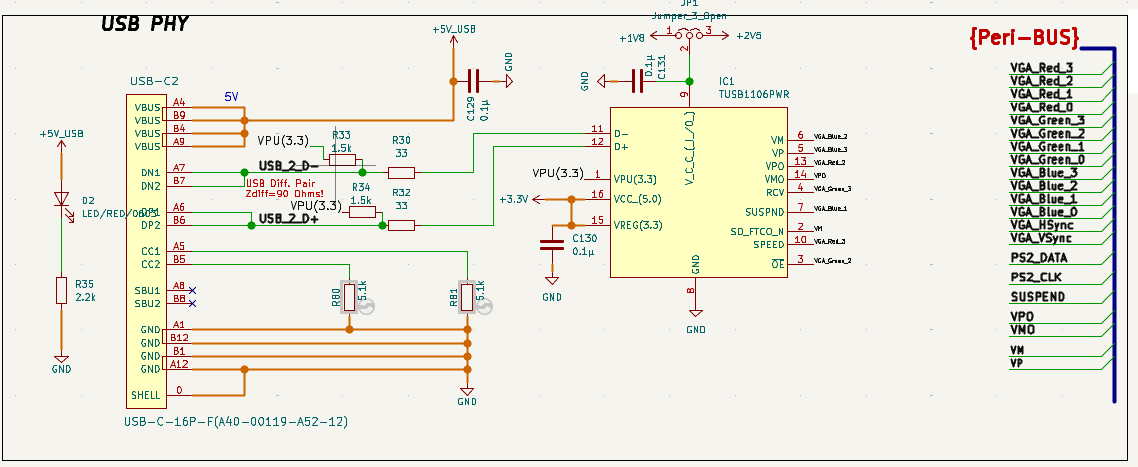
\includegraphics[width=0.9\textwidth]{assets/USB_PHY_Schaltplan.png}
	\caption{Schematic des USB-2.0-PHY (TUSB1106)}
	\label{fig:usb_phy_schematic}
\end{figure}

\textbf{Schematic des ISO/IEC-7816-Interfaces}

Für das ISO/IEC-7816-3-konforme Interface wurden die Signale VCC, GND, CLK, RST und I/O vorgesehen. Die Versorgungsspannung ist zwischen Class~A mit 5~V, Class~B mit 3~V und Class~C mit 1,8~V umschaltbar.

% Abbildung: ISO/IEC-7816-3-Interface Schematic -- Datei fehlt aktuell
% \begin{figure}[H]
% 	\centering
% 	\includegraphics[width=0.9\textwidth]{assets/iso7816_schematic.png}
% 	\caption{Schematic des ISO/IEC-7816-3-Interfaces}
% 	\label{fig:iso7816_schematic}
% \end{figure}

\textbf{Layout}
\begin{itemize}
	\item Umsetzung des USB-PHY einschließlich differentiell geroutetem D+/D--Pair.
	\item Umsetzung des ISO/IEC-7816-Interfaces mit VCC-Umschaltpfad.
	\item Umsetzung der USB-C-Power-Topologie mit der Schottky-Diode B340.
\end{itemize}

\begin{figure}[H]
	\centering
	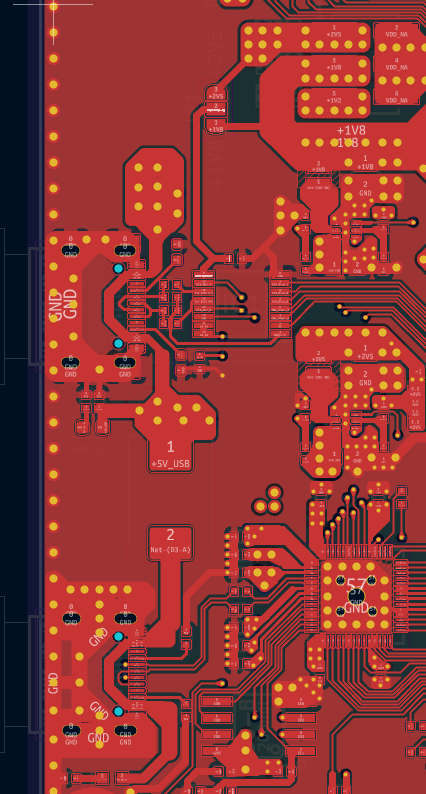
\includegraphics[width=0.8\textwidth]{assets/USB_PHY_platine_layerview.png}
	\caption{Layout USB-PHY mit differentiellem D+/D--Pair}
	\label{fig:layout_usb_phy}
\end{figure}

% Abbildung: ISO/IEC-7816-Interface Layout -- Datei fehlt aktuell
% \begin{figure}[H]
% 	\centering
% 	\includegraphics[width=0.8\textwidth]{assets/layout_iso7816.png}
% 	\caption{Layout ISO/IEC-7816-Interface mit VCC-Switching-Pfad}
% 	\label{fig:layout_iso7816}
% \end{figure}

% Abbildung: USB-C-Power-Topologie Layout -- Datei fehlt aktuell
% \begin{figure}[H]
% 	\centering
% 	\includegraphics[width=0.8\textwidth]{assets/layout_usb_power.png}
% 	\caption{Layout USB-C-Power-Topologie mit Schottky-Diode B340}
% 	\label{fig:layout_usb_power}
% \end{figure}

\textbf{Funktionsweise des TUSB1106}

Der TUSB1106\footnote{Texas Instruments, \textit{Advanced Universal Serial Bus Transceivers}, Datenblatt SCAS818E: \url{https://www.ti.com/lit/gpn/TUSB1106}} ist ein USB-2.0-konformer Transceiver (PHY), der die analoge Signalebene des USB-Busses von der digitalen Protokolllogik trennt: Die Serial Interface Engine (SIE) mit NRZI-Codierung, Bitstuffing, PID-Verarbeitung und CRC-Berechnung läuft im GateMate-FPGA, der Baustein selbst übernimmt ausschließlich Pegelwandlung, Bustreiber und Empfänger. Die digitale Schnittstelle wird über eine eigene I/O-Versorgung (VCC(I/O), 1,65 bis 3,6\,V) versorgt und ist damit direkt mit den 1,8-V-I/O-Bänken des GateMate kompatibel; dabei darf VCC(I/O) laut Datenblatt nie die Spannung von Vreg(3.3) überschreiten. Die analoge Seite wird entweder über den integrierten, abschaltbaren 5-V-zu-3,3-V-Regler direkt aus VBUS gespeist (VCC(5.0): 4 bis 5,5\,V) oder im Regler-Bypass-Modus aus einer vorhandenen 3,3-V-Versorgung. Über SUSPND = 1 lässt sich ein Low-Power-Zustand anfordern, in dem RCV auf Low gezogen wird; das Aufwecken erfolgt durch ein K-Signal mit einer Dauer von 1 bis 15\,ms (Remote-Wakeup).

\begin{table}[H]
	\centering
	\begin{tabular}{|l|l|p{8.2cm}|}
		\hline
		\textbf{Signal} & \textbf{Richtung}      & \textbf{Funktion (laut Datenblatt)}                                                            \\ \hline
		OE              & FPGA $\rightarrow$ PHY & Treiber-Freigabe, aktiv low: 0 = Senden auf D+/D--, 1 = Empfang (Bus freigegeben)              \\ \hline
		SPEED           & FPGA $\rightarrow$ PHY & Slew-Rate-Wahl gemäß Geschwindigkeit: 1 = Full-Speed (12\,Mbit/s), 0 = Low-Speed (1,5\,Mbit/s) \\ \hline
		VPO/VMO         & FPGA $\rightarrow$ PHY & Differenzielle Treiberdaten für D+ und D--; beide Low erzeugt SE0                              \\ \hline
		RCV             & PHY $\rightarrow$ FPGA & Empfangener NRZI-Bitstrom; Pegel bleibt stabil während SE0, Low bei Suspend                    \\ \hline
		VP/VM           & PHY $\rightarrow$ FPGA & Single-Ended-Empfänger an D+ und D--: SE0-Erkennung, Fehler- und VBUS-Sensing                  \\ \hline
		SUSPND          & FPGA $\rightarrow$ PHY & 1 = Low-Power-Zustand (RCV = Low), 0 = Normalbetrieb                                           \\ \hline
	\end{tabular}
	\caption{Digitale Schnittstelle des TUSB1106 an das FPGA}
	\label{tab:tusb_signals}
\end{table}

Während Senden (OE = 0) schaltet der PHY die an VPO und VMO anliegenden Pegel direkt auf D+ und D-- durch (Tabelle~\ref{tab:tusb_drive}); der Zustand VPO = VMO = 0 erzeugt einen Single-Ended-Zero (SE0). Mit OE = 1 gibt der PHY den Bus frei: Die differentielle Empfangsrichtung liefert den NRZI-Bitstrom an RCV, während die beiden Single-Ended-Empfänger mit Hysterese die Einzelleiter-Pegel an VP und VM ausgeben. Dabei entspricht RCV = H dem J-Zustand und RCV = L dem K-Zustand; VP = VM = L kennzeichnet SE0, VP = VM = H signalisiert fehlende Versorgung und damit eine VBUS-Unterbrechung. Da RCV während eines SE0 stabil auf dem letzten Pegel bleibt, lassen sich Bus-Reset und Paketende auch ohne Takt-Rückgewinnung erkennen.

\begin{table}[H]
	\centering
	\begin{tabular}{|l|l|l|}
		\hline
		\textbf{VPO} & \textbf{VMO} & \textbf{Buszustand (Full-Speed)} \\ \hline
		0            & 0            & SE0 (Paketende)                  \\ \hline
		0            & 1            & K (differenzielle 0)             \\ \hline
		1            & 0            & J (differenzielle 1 / Idle)      \\ \hline
		1            & 1            & unzulässiger Zustand             \\ \hline
	\end{tabular}
	\caption{Sendefunktion des TUSB1106 (Datenblatt, Tab.~4)}
	\label{tab:tusb_drive}
\end{table}

Die Soft-Connect-Funktion wird über SOFTCON und den Pin Vpu(3.3) gesteuert: Bei SOFTCON = 1 legt der Baustein die Pull-up-Versorgung an Vpu an, wodurch der externe 1,5-k$\Omega$-Widerstand D+ gegen 3,3\,V zieht und der Host den Device-Anschluss am Übergang von SE0 nach J erkennt. Bei SOFTCON = 0 bleibt Vpu hochohmig (null Pull-up-Strom) und das Gerät erscheint vom Bus abgekoppelt. In unserem Design wird der externe 1,5-k$\Omega$-Pull-up an D+ über SOFTCON und die Vpu-Versorgung freigegeben; ist der Pull-up aktiv, erkennt der Host das Modul als Full-Speed-Device.

Die physikalische Schicht des USB-2.0-Standards\footnote{USB Implementers Forum, \textit{Universal Serial Bus Specification Rev.~2.0}: \url{https://www.usb.org/document-library/usb-20-specification}} überträgt Daten LSB-zuerst im NRZI-Code: Eine logische 0 erzeugt einen Pegelwechsel auf dem Bus, eine logische 1 lässt den Pegel unverändert. Daraus ergeben sich für die FPGA-Seite die folgenden Randbedingungen:
\begin{itemize}
	\item Jedes Paket beginnt mit dem SYNC-Feld 00000001 (LSB zuerst), das auf dem Bus als Wechselfolge KJKJKJKK erscheint und dem Empfänger Takt und Bitphase liefert.
	\item Das Paketende (EOP) wird durch 2 Bitzeiten SE0 gefolgt von 1 Bitzeit J signalisiert.
	\item Nach sechs aufeinanderfolgenden Einsen fügt der Sender ein Stuff-Bit 0 ein, damit der Empfänger aus den Pegelwechseln den Takt zurückgewinnen kann; die Eins, die das SYNC-Muster beendet, zählt dabei als erste Eins.
	\item Datenpakete sind mit CRC16 (Polynom $x^{16}+x^{15}+x^{2}+1$, Initialwert FFFF), Tokenpakete mit CRC5 ($x^{5}+x^{2}+1$) geschützt; die Prüfbits werden jeweils invertiert übertragen.
	\item Auf einen Token antwortet das Device innerhalb der Turnaround-Zeit von maximal 7,5 Bitzeiten.
	\item Der 1,5-k$\Omega$-Pull-up an D+ kennzeichnet ein Full-Speed-Device; der Host erkennt Bus-Resets beziehungsweise das Gerät über die SE0- und J-Zustände.
\end{itemize}
Elektrisch spezifiziert das Datenblatt eine Treiberimpedanz von 34 bis 44\,$\Omega$ inklusive der externen 33-$\Omega$-Serienwiderstände, Anstiegs- und Abfallzeiten von 4 bis 20\,ns (Full-Speed), eine Laufzeit von D+/D-- zu RCV von maximal 15\,ns sowie eine ESD-Festigkeit von ±15\,kV (HBM) an den Bus-Pins.

\textbf{USB-Testmodul in VHDL}

Um den TUSB1106 direkt beim Bring-up ansteuern und prüfen zu können, wurde ein Testmodul in VHDL entworfen, das die Funktion der SIE in minimierter Form nachbildet. Es greift damit die Stufe 3 des Bringup-Plans auf und erweitert sie um die Protokollebene, und es erlaubt drei Verifikationsstufen: (1) ein reiner Sendetest mit periodischen Testpaketen, verifizierbar über Oszilloskop und Logic-Analyzer an D+/D--, (2) ein Token-Responder, der auf adressierte IN-Polls mit NAK beziehungsweise mit einem HID-Report antwortet und sich über einen USB-Analyzer beobachten lässt, und (3) nach Ergänzung der Enumerations-Logik die vollwertige Erkennung als USB-Device (siehe Ausblick). Das Modul ist als synthetisierbares VHDL-93 gehalten, lässt sich mit GHDL simulieren und über die GHDL-Yosys-Anbindung auch in die Cologne-Chip-Toolchain überführen. Simulation und Synthese sind zum aktuellen Stand noch nicht durchgeführt.

\begin{itemize}
	\item \textbf{Bittakt:} Aus dem 48-MHz-Systemtakt erzeugt ein Teiler alle vier Zyklen ein Bittakt-Enable (48\,MHz / 4 = 12\,Mbit/s); die Bitphase wird beim Empfang am SYNC-Muster eingenommen.
	\item \texttt{usb\_tx}: Serialisiert SYNC, PID, Nutzdaten und CRC16, wendet on-the-fly das Bitstuffing an und codiert NRZI; das Paketende wird durch SE0 signalisiert.
	\item \texttt{usb\_rx}: Sucht das SYNC-Muster, decodiert NRZI mit Unstuffing, prüft die PID-Komplementbits und decodiert IN-Token (Adresse, Endpoint).
	\item \texttt{usb\_dev}: Erkennt den Bus-Reset (SE0 $\geq$ 2,5\,$\mu$s), antwortet auf IN-Token am Tastatur-Endpoint nach 4 Bitzeiten Turnaround mit einem 8-Byte-HID-Report (Taste \texttt{a} über den Board-Taster) oder mit NAK.
	\item Die Ports entsprechen 1:1 den Constraints der \texttt{.ccf}-Datei (\texttt{usb\_rcv}, \texttt{usb\_vpo}, \texttt{usb\_vmo}, \texttt{usb\_vp}, \texttt{usb\_vm}, \texttt{usb\_oe}); \texttt{usb\_speed} ist fest auf 1 (Full-Speed) und \texttt{usb\_susp} auf 0 (Normalbetrieb) gelegt.
\end{itemize}

Der Sendeteil mit NRZI-Codierung, Bitstuffing und CRC16:

\begin{verbatim}
-- usb_tx.vhd: Sendeteil des USB-PHY-Testmoduls (Full-Speed, 12 Mbit/s)
-- Ansteuerung des TUSB1106 gemaess Datenblatt Tab. 4: OE = '0' aktiviert
-- den Treiber, VPO = D+, VMO = D-; VPO = VMO = '0' erzeugt SE0 (EOP)
library ieee;
use ieee.std_logic_1164.all;

entity usb_tx is
    port (
        clk      : in  std_logic;                    -- 48-MHz-Systemtakt
        rst      : in  std_logic;
        bit_en   : in  std_logic;                    -- Bittakt-Enable (12 MHz)
        start    : in  std_logic;                    -- Uebertragung starten
        pid      : in  std_logic_vector(7 downto 0); -- z. B. DATA1 = 0x4B
        payload  : in  std_logic_vector(63 downto 0);
        plen     : in  natural range 0 to 8;         -- Nutzlaenge in Byte
        send_crc : in  std_logic;                    -- '1' = CRC16 anhaengen
        done     : out std_logic;
        phy_oe   : out std_logic;
        phy_vpo  : out std_logic;                    -- VPO = D+
        phy_vmo  : out std_logic                     -- VMO = D-
    );
end entity;

architecture rtl of usb_tx is
    type state_t is (IDLE, SYNC, PKT, SE0_A, SE0_B, GAP);
    signal state : state_t := IDLE;
    signal nbits : natural range 8 to 88;
    signal idx   : natural range 0 to 87 := 0;
    signal ones  : natural range 0 to 6 := 0;      -- Stuffing-Zaehler
    signal stuff : std_logic := '0';               -- naechstes Bit: Stuff-Bit
    signal nrzi  : std_logic := '1';               -- Buspegel (1 = J, 0 = K)
    signal crc   : std_logic_vector(15 downto 0);

    -- CRC16 der USB-Spezifikation: G(x) = x^16 + x^15 + x^2 + 1,
    -- Initialwert FFFF, LSB zuerst, Pruefbits werden invertiert gesendet
    function crc16_next(c : std_logic_vector(15 downto 0);
                        d : std_logic) return std_logic_vector is
        variable fb : std_logic;
        variable n  : std_logic_vector(15 downto 0);
    begin
        fb    := c(0) xor d;
        n(0)  := c(1) xor fb;
        n(1)  := c(2);
        n(2)  := c(3);
        n(3)  := c(4);
        n(4)  := c(5);
        n(5)  := c(6);
        n(6)  := c(7);
        n(7)  := c(8);
        n(8)  := c(9);
        n(9)  := c(10);
        n(10) := c(11);
        n(11) := c(12);
        n(12) := c(13);
        n(13) := c(14) xor fb;
        n(14) := c(15);
        n(15) := fb;
        return n;
    end function;
begin

    done <= '1' when state = GAP else '0';

    -- Treiberansteuerung: Idle = J (VPO = '1', VMO = '0'), SE0 im EOP
    phy_oe  <= '0' when state /= IDLE else '1';
    phy_vpo <= '0' when state = SE0_A or state = SE0_B else nrzi;
    phy_vmo <= '0' when state = SE0_A or state = SE0_B else not nrzi;

    process (clk)
        variable bitv : std_logic;
    begin
        if rising_edge(clk) then
            if rst = '1' then
                state <= IDLE;
                nrzi  <= '1';
                idx   <= 0;
                ones  <= 0;
                stuff <= '0';
                crc   <= (others => '0');
            elsif bit_en = '1' then
                case state is

                    when IDLE =>
                        if start = '1' then
                            nbits <= 8 + plen * 8 + 16 when send_crc = '1'
                                     else 8 + plen * 8;
                            idx   <= 0;
                            ones  <= 0;
                            stuff <= '0';
                            crc   <= x"FFFF";
                            state <= SYNC;
                        end if;

                    when SYNC =>                  -- SOP: 00000001 -> KJKJKJKK
                        if idx < 7 then
                            bitv := '0';
                        else
                            bitv := '1';
                        end if;
                        if bitv = '0' then
                            nrzi <= not nrzi;
                        end if;
                        if idx = 7 then
                            idx   <= 0;
                            ones  <= 1;               -- Sync-Eins zaehlt mit (Spec 7.1.9)
                            stuff <= '0';
                            state <= PKT;
                        else
                            idx <= idx + 1;
                        end if;

                    when PKT =>                   -- PID, Nutzdaten, CRC16
                        if stuff = '1' then       -- erzwungenes Stuff-Bit '0'
                            bitv  := '0';
                            stuff <= '0';
                            ones  <= 0;
                            if idx = nbits - 1 then   -- Stuff-Bit war letztes Bit
                                state <= SE0_A;
                            end if;
                        else
                            if idx < 8 then
                                bitv := pid(idx);
                            elsif idx < 8 + plen * 8 then
                                bitv := payload(idx - 8);
                                crc  <= crc16_next(crc, bitv);
                            else
                                bitv := not crc(idx - 8 - plen * 8);
                            end if;
                            if bitv = '1' then
                                if ones = 5 then
                                    stuff <= '1';  -- 6 Einsen -> Stuff-Bit
                                    ones  <= 6;
                                else
                                    ones <= ones + 1;
                                end if;
                            else
                                ones <= 0;
                            end if;
                            if idx = nbits - 1 then
                                if not (bitv = '1' and ones = 5) then
                                    state <= SE0_A;
                                end if;           -- sonst folgt erst das Stuff-Bit
                            else
                                idx <= idx + 1;
                            end if;
                        end if;
                        if bitv = '0' then
                            nrzi <= not nrzi;
                        end if;

                    when SE0_A =>                 -- EOP: 2 Bitzeiten SE0
                        state <= SE0_B;

                    when SE0_B =>
                        nrzi  <= '1';             -- Rueckkehr nach J (Idle)
                        state <= GAP;

                    when GAP =>                   -- 1 Bitzeit J, dann frei
                        state <= IDLE;
                end case;
            end if;
        end if;
    end process;

end architecture;
\end{verbatim}

Der Empfangsteil (Auszug) mit SYNC-Jagd, NRZI-Decodierung, Unstuffing und Token-Decodierung:

\begin{verbatim}
-- usb_rx.vhd (Auszug): RCV liefert den NRZI-Strom, VP/VM die Single-Ended-
-- Pegel zur SE0-Erkennung (Datenblatt Tab. 5). Die Bitphase wird am SYNC-
-- Muster eingenommen; token_in wird nur fuer gueltige IN-Token erzeugt.
library ieee;
use ieee.std_logic_1164.all;
use ieee.numeric_std.all;

entity usb_rx is
    port (
        clk        : in  std_logic;
        rst        : in  std_logic;
        bit_en     : in  std_logic;
        phy_rcv    : in  std_logic;          -- RCV: NRZI-Bitstrom (Idle = J)
        phy_vp     : in  std_logic;          -- VP: Single-ended D+
        phy_vm     : in  std_logic;          -- VM: Single-ended D-
        se0        : out std_logic;
        token_in   : out std_logic;          -- gueltiger IN-Token empfangen
        token_addr : out natural range 0 to 127;
        token_endp : out natural range 0 to 15
    );
end entity;

architecture rtl of usb_rx is
    type state_t is (HUNT, PID, TOKEN);
    signal state : state_t := HUNT;
    signal prev  : std_logic := '1';
    signal sreg  : std_logic_vector(15 downto 0) := (others => '0');
    signal pid_l : std_logic_vector(7 downto 0);
    signal cnt   : natural range 0 to 15 := 0;
    signal ones  : natural range 0 to 6 := 0;
begin

    se0 <= '1' when phy_vp = '0' and phy_vm = '0' else '0';

    process (clk)
        variable dbit : std_logic;             -- decodiertes Datenbit
        variable v    : std_logic_vector(15 downto 0);
    begin
        if rising_edge(clk) then
            if rst = '1' then
                state <= HUNT;
                prev  <= '1';
                pid_l <= x"00";
            elsif bit_en = '1' then
                token_in <= '0';
                -- NRZI-Decodierung: Pegelwechsel = '0', kein Wechsel = '1'
                if phy_rcv /= prev then
                    dbit := '0';
                else
                    dbit := '1';
                end if;
                prev := phy_rcv;

                case state is

                    when HUNT =>               -- SYNC-Datenbits 0x80, LSB zuerst
                        v    := dbit & sreg(15 downto 1);
                        sreg <= v;
                        if v(15 downto 8) = x"80" then
                            cnt   <= 0;
                            ones  <= 1;        -- Sync-Eins zaehlt mit (Spec 7.1.9)
                            state <= PID;
                        end if;

                    when PID =>
                        if ones = 6 then       -- Stuff-Bit verwerfen
                            ones <= 0;
                        else
                            v    := dbit & sreg(15 downto 1);
                            sreg <= v;
                            ones <= ones + 1 when dbit = '1' else 0;
                            if cnt = 7 then
                                if v(11 downto 8) = not v(15 downto 12) then
                                    pid_l <= v(15 downto 8);  -- PID-Byte merken
                                    cnt   <= 0;   -- PID-Komplement ok
                                    state <= TOKEN;
                                else
                                    state <= HUNT;
                                end if;
                            else
                                cnt <= cnt + 1;
                            end if;
                        end if;

                    when TOKEN =>
                        if ones = 6 then
                            ones <= 0;
                        else
                            v    := dbit & sreg(15 downto 1);
                            sreg <= v;
                            ones <= ones + 1 when dbit = '1' else 0;
                            if cnt = 15 then     -- 7 Adresse + 4 EP + 5 CRC5
                                if pid_l = x"69" then          -- IN-Token
                                    token_addr <= to_integer(unsigned(v(6 downto 0)));
                                    token_endp <= to_integer(unsigned(v(10 downto 7)));
                                    token_in   <= '1';
                                end if;        -- CRC5 im Testmodul ungeprueft
                                cnt   <= 0;
                                state <= HUNT;
                            else
                                cnt <= cnt + 1;
                            end if;
                        end if;
                end case;
            end if;
        end if;
    end process;

end architecture;
\end{verbatim}

Die Transaktionslogik des Testmoduls (Auszug): Nach einem IN-Token an die eigene Adresse antwortet das Modul nach Ablauf der Turnaround-Zeit mit einem 8-Byte-HID-Tastatur-Report oder mit NAK:

\begin{verbatim}
-- usb_dev.vhd (Auszug): Taster gedrueckt -> DATA1 mit HID-Report
-- (0x04 = Taste 'a'), sonst NAK; Bus-Reset setzt die Adresse zurueck.
library ieee;
use ieee.std_logic_1164.all;

entity usb_dev is
    port (
        clk        : in  std_logic;
        rst        : in  std_logic;
        bit_en     : in  std_logic;
        se0        : in  std_logic;            -- vom usb_rx
        tx_done    : in  std_logic;            -- von usb_tx
        token_in   : in  std_logic;
        token_addr : in  natural range 0 to 127;
        token_endp : in  natural range 0 to 15;
        btn        : in  std_logic;            -- Taster (2FF-synchronisiert)
        start      : out std_logic;
        pid        : out std_logic_vector(7 downto 0);
        payload    : out std_logic_vector(63 downto 0);
        plen       : out natural range 0 to 8;
        send_crc   : out std_logic
    );
end entity;

architecture rtl of usb_dev is
    -- HID-Report: Modifier, reserviert, 6 Keycodes (0x04 = Taste 'a')
    constant KEY_A : std_logic_vector(63 downto 0) := x"0000000000040000";
    signal dev_addr : natural range 0 to 127 := 0;
    signal pend     : std_logic := '0';
    signal gap      : natural range 0 to 4 := 4;
    signal se0_cnt  : natural range 0 to 31 := 0;
begin

    process (clk)
    begin
        if rising_edge(clk) then
            if rst = '1' then
                dev_addr <= 0;
                pend     <= '0';
                gap      <= 4;
                se0_cnt  <= 0;
                start    <= '0';
            elsif bit_en = '1' then
                start <= '0';
                -- Bus-Reset: SE0 laenger als 2,5 us = 30 Bitzeiten
                if se0 = '1' then
                    if se0_cnt = 30 then
                        dev_addr <= 0;
                        pend     <= '0';
                    else
                        se0_cnt <= se0_cnt + 1;
                    end if;
                else
                    se0_cnt <= 0;
                end if;

                -- IN-Token am Tastatur-Endpoint (EP1): Turnaround abwarten
                if token_in = '1' and token_addr = dev_addr
                   and token_endp = 1 then
                    gap <= 0;
                elsif gap /= 4 then
                    if gap = 3 then
                        start <= '1';           -- Antwortpaket senden
                        gap   <= 4;
                    else
                        gap <= gap + 1;
                    end if;
                end if;

                -- Tastendruck vormerken, nach gesendeter Antwort freigeben
                if btn = '1' then
                    pend <= '1';
                elsif tx_done = '1' then
                    pend <= '0';
                end if;
            end if;
        end if;
    end process;

    -- ausstehender Tastendruck: DATA1 + Report (mit CRC16), sonst NAK
    pid      <= x"4B" when pend = '1' else x"5A";
    payload  <= KEY_A when pend = '1' else x"0000000000000000";
    plen     <= 8 when pend = '1' else 0;
    send_crc <= pend;

end architecture;
\end{verbatim}

Die drei Blöcke werden im Top-Level instanziiert und an die Constraints der \texttt{.ccf}-Datei angebunden; der Bittakt-Enable ergibt sich aus einem Teiler 48\,MHz / 4, \texttt{usb\_speed} ist fest auf 1 (Full-Speed) und \texttt{usb\_susp} auf 0 (Normalbetrieb) gelegt. Die vollständigen, synthetisierbaren Quelltexte samt Top-Level und Constraints liegen im Repository unter \texttt{software/usb\_phy\_test/}. Für den reinen Sendetest ohne Host wird statt des Responders ein periodischer Paketgenerator an \texttt{tx\_start} gelegt; die Verifikation von Pegeln, Stuffing- und EOP-Timing erfolgt dann über Oszilloskop bzw. Logic-Analyzer an D+/D--. \texttt{usb\_susp} bleibt dabei auf 0, da Suspend erst mit der vollständigen Enumerationslogik sinnvoll nutzbar ist.

\textbf{Ausblick: Vom Testmodul zum USB-Device}

Als nächster Schritt (nächstes Semester) soll aus dem Testmodul ein vollwertiges USB-Device werden. Es fehlt die Enumerationslogik für die Kontrollübertragungen am Default-Endpoint 0:
\begin{enumerate}
	\item Erkennung des Bus-Resets (SE0 $\geq$ 2,5\,$\mu$s) und Zurücksetzen der Device-Adresse auf 0.
	\item Empfang der SETUP-Transaktionen mit 8-Byte-Request und Antworten mit ACK; Decodierung von \texttt{SET\_ADDRESS}, \texttt{GET\_DESCRIPTOR} und \texttt{SET\_CONFIGURATION}.
	\item Bereitstellung von Device-, Config-, Interface- und Endpoint-Deskriptoren als ROM-Konstanten im FPGA.
	\item Verwaltung des DATA-Toggles in den Daten- und Statusphasen der Kontrollübertragungen.
\end{enumerate}
Damit steht die Wahl des Minimalbeispiels, mit dem die Kommunikation über den Transceiver nachgewiesen werden kann:
\begin{itemize}
	\item \textbf{Virtual COM Port (CDC-ACM):} Das empfohlene Minimalbeispiel: Das Device enumeriert als virtuelle serielle Schnittstelle, und ein Echo-Demo auf dem FPGA spiegelt empfangene BULK-Daten zurück. Damit sind Enumeration und bidirektionale BULK-Transfers vollständig bewiesen, bei vergleichsweise geringem Aufwand.
	\item \textbf{HID-Tastatur:} Der TX-Pfad samt 8-Byte-HID-Report existiert im Testmodul bereits; es fehlen nur die Enumerations-FSM und der HID-Report-Deskriptor. Das Gerät täte dann am PC so, als wäre es eine Tastatur.
	\item \textbf{USB-Massenspeicher (MSC):} Die aufwendigste Variante, da zusätzlich das Bulk-Only-Transport-Protokoll (BOT) und ein SCSI-Befehlssatz (INQUIRY, READ CAPACITY, READ10/WRITE10) umzusetzen sind. Sinnvoll als Folgeprojekt, sobald CDC-ACM steht.
\end{itemize}
Mit Blick auf die Smart-Card-Anwendung ist langfristig die USB-Geräteklasse CCID das Ziel, über die ein Host mit Chipkartenlesern kommuniziert; CDC-ACM und HID dienen dabei als Verifikationsschritte auf dem Weg dorthin.
Als Referenz für die Umsetzung bietet sich die offene Verilog-Implementierung \texttt{usb\_cdc}\footnote{\url{https://github.com/ulixxe/usb_cdc}} an; die Verifikation erfolgt über \texttt{usbmon}/Wireshark auf Host-Seite sowie Logic-Analyzer an D+/D--. Voraussetzung für alle Schritte ist ein stabiler Takt für das FPGA (siehe Abschnitt zur fehlenden Clock), da sowohl die 12-Mbit/s-Bitrate als auch die Erkennung von Reset, Suspend und Resume eine genaue Zeitbasis benötigen.

\textbf{Status und offene Punkte}

Zum Stand der Umsetzung: Schaltbild und Layout des USB-PHY sind umgesetzt und eingecheckt, eine Kommunikation über den TUSB1106 wurde jedoch noch nicht getestet. Die folgenden Punkte sind offen und müssen vor bzw. während der Inbetriebnahme geklärt werden:
\begin{itemize}
	\item R33 (1,5-k$\Omega$-Pull-up an D--) prüfen: Für Full-Speed darf nur D+ (R34) den Pull-up nach Vpu führen; ein Pull-up auf D-- erzeugt im Idle-Zustand einen unzulässigen Buszustand (SE1, beide Leitungen auf High) und verhindert die Geräteenkennung.
	\item SOFTCON (SD\_FTCO\_N) ist als neuntes Signal geroutet, fehlt aber noch in den Constraints; es muss als FPGA-Pin angebunden oder fest auf High gelegt werden, sonst zieht der 1,5-k$\Omega$-Pull-up D+ nicht hoch.
	\item Pinzuordnung von VPO (Pin 13), VMO (Pin 14) und RCV (Pin 4) im Symbol gegen das Datenblatt prüfen.
	\item Anbindung von Vreg(3.3) an die 3,3-V-Schiene im Regler-Bypass-Modus prüfen; laut Datenblatt müssen VCC(5.0) und Vreg(3.3) verbunden sein.
	\item Die differentielle Impedanz von 90~$\Omega$ auf dem D+/D---Paar ist layoutseitig ausgelegt, aber messtechnisch nicht verifiziert.
	\item Das VHDL-Testmodul ist quelltextseitig fertig, aber noch nicht simuliert, synthetisiert oder auf der Hardware getestet.
\end{itemize}

\textbf{Zusammenarbeit mit Fynn}
\begin{itemize}
	\item Iterative Abstimmung der Schematic-Blöcke für die Integration in KiCad.
	\item Gemeinsame Design-Reviews zu Footprints, Bauteilgrößen und Routing.
	\item Das finale PCB-Layout, den DRC und den Arduino-Header hat Fynn übernommen.
\end{itemize}
\newpage
\section{Bestellung und BOM-Management | Timo}

\textbf{Bill of Materials (BOM) und Sourcing-Strategie}
\begin{itemize}
	\item \textbf{Generische zu spezifische BOM:} Ausgangspunkt meiner Arbeit war die generische Bill of Materials des Olimex-Evaluationsboards. Da unser PCB-Design jedoch stark von der Referenz abwich (z.B. durch den TUSB1106 PHY, das ISO-Interface und debloatete Peripherie), musste diese Stückliste systematisch bereinigt und auf unser spezifisches Design zugeschnitten werden. Die finale BOM umfasst 79 einzigartige Positionen mit insgesamt knapp 800 Einzelbauteilen für drei Boards.
	\item \textbf{Distributor-Konsolidierung:} Da der GateMate-FPGA ein recht exklusiver Baustein ist, war DigiKey die einzige große Beschaffungsplattform, die diesen Chip (sowie den IBEX-Softcore-kompatiblen Flash) im Sortiment anbot. Um zusätzliche Versandkosten und logistischen Aufwand durch mehrere Lieferanten zu vermeiden, wurde die komplette BOM mithilfe von Octopart so umgearbeitet, dass alle Komponenten zentral über DigiKey bestellt werden konnten.
	\item \textbf{Kostenoptimierung durch Packaging:} Bei der Recherche fiel auf, dass für bestimmte Widerstände (z.B. den 1,05\,k$\Omega$ Widerstand \texttt{RC0402FR-071K05L}) sogenannte \textit{Digi-Reel} Artikelnummern (Suffix \texttt{-DKR-ND}) hinterlegt waren, für die der Distributor eine Abrollgebühr von ca. 7\,\$ pro Rolle verlangt. Durch gezieltes Umschlüsseln auf \textit{Cut-Tape} Varianten (Suffix \texttt{-CT-ND}) konnten diese versteckten Kosten eliminiert werden.
\end{itemize}

\section{Component Substitution | Timo}
Viele ursprünglich vorgesehene Bauteile waren abgekündigt oder kurzfristig nicht lieferbar (Preis = 0\,€ im System). Daher mussten anhand technischer Datenblätter passende Ersatzkomponenten ermittelt werden. Wichtige Kriterien waren hierbei exakte Funktionalität, Pin-Kompatibilität, identische Gehäuseformen (Footprints) sowie die strikte Einhaltung der Toleranzen.

Ein zentrales Beispiel für diese Substitution war der 47\,$\mu$F Kondensator für die Spannungsstabilisierung:
\begin{table}[H]
	\centering
	\begin{tabular}{|l|l|l|}
		\hline
		\textbf{Parameter}       & \textbf{Ursprünglich (Nicht lieferbar)} & \textbf{Gewählte Alternative}  \\ \hline
		Hersteller               & Samsung Electro-Mechanics               & Murata Electronics             \\ \hline
		Part Number (MPN)        & \texttt{CL21A476MQYNNNE}                & \texttt{GRM21BR61A476ME15}     \\ \hline
		DigiKey SKU              & \texttt{1276-1852-1-ND}                 & \texttt{490-9961-1-ND}         \\ \hline
		Kapazität \& Footprint   & 47\,$\mu$F, 0805 (2012 Metric)          & 47\,$\mu$F, 0805 (2012 Metric) \\ \hline
		Dielektrikum \& Toleranz & X5R, $\pm$20\%                          & X5R, $\pm$20\%                 \\ \hline
		Spannungsfestigkeit      & 6.3\,V                                  & \textbf{10.0\,V}               \\ \hline
	\end{tabular}
	\caption{Vergleich der Kondensator-Substitution}
	\label{tab:cap_subst}
\end{table}
Wie aus Tabelle~\ref{tab:cap_subst} ersichtlich, erfüllt die Alternative nicht nur alle Footprint-Vorgaben, sondern bietet mit 10\,V eine höhere Spannungsfestigkeit, was das Derating verbessert und die Zuverlässigkeit der Schaltung erhöht. Ähnliche Substitutionen wurden unter anderem für 2,2\,k$\Omega$ Widerstände (Wechsel auf Vishay \texttt{CRCW04022K20FKED}) durchgeführt.

\vspace{1em}
\textbf{Mengenplanung und Reservestrategie}

Die finale BOM wurde für die Bestückung von drei Prototypen-Platinen kalkuliert. Da bei der Handbestückung und dem Reflow-Löten im Labor mit Schwund oder Fehlern gerechnet werden muss, wurde eine systematische Reservestrategie angewandt:
\begin{itemize}
	\item \textbf{Passive SMD-Bauteile (0402/0603):} Für diese sehr kleinen und günstigen Komponenten wurde eine großzügige Reserve von +15\,\% der benötigten Menge, mindestens jedoch +5 Stück als absoluter Puffer, eingeplant.
	\item \textbf{Aktive Bauteile \& ICs:} Bei kostenintensiveren Bauteilen wie dem USB-PHY (TUSB1106), den LDOs oder dem GateMate-FPGA wurde knapper kalkuliert. Hier galt die strikte Regel: Exakte Menge für 3 Boards \textbf{plus genau 1 Ersatz-IC} pro Bauteiltyp, um im Fehlerfall sofort einen Chip austauschen zu können, ohne das Budget unnötig zu belasten.
\end{itemize}

\section{Festlegung der Pinbelegung und Constraints | Timo}

Um den externen USB-2.0-PHY (TUSB1106) an den GateMate-FPGA anzubinden, musste eine geeignete Pinbelegung (Pin Assignment) definiert werden. Da das Routing auf der Platine durch den Formfaktor stark eingeschränkt war, wurden die digitalen Signale (VM, VP, VPO, VMO, RCV, OE) auf die Pins des Peri-BUS geroutet, die ursprünglich für die \texttt{VGA\_Red} und \texttt{VGA\_Blue} Signale des Olimex-Boards vorgesehen waren.

Dies ermöglichte ein signalintegres, kreuzungsfreies Routing. Für die Synthese und das anschließende Place-\&-Route (P\&R) mit der Cologne Chip Toolchain habe ich die entsprechenden Constraints in der \texttt{.ccf}-Datei (Cologne Chip Constraint File) wie folgt definiert:

\begin{verbatim}
# USB PHY TUSB1106 Pin Constraints (via Olimex VGA/Peri-BUS)
Pin_in  "usb_rcv"   Loc = "IO_WA_A0";  # Routed via VGA_Red_0
Pin_out "usb_vpo"   Loc = "IO_WA_A1";  # Routed via VGA_Red_1
Pin_out "usb_vmo"   Loc = "IO_WA_A2";  # Routed via VGA_Red_2
Pin_in  "usb_vp"    Loc = "IO_WA_B0";  # Routed via VGA_Blue_0
Pin_in  "usb_vm"    Loc = "IO_WA_B1";  # Routed via VGA_Blue_1
Pin_out "usb_oe"    Loc = "IO_WA_B2";  # Routed via VGA_Blue_2
Pin_in  "usb_susp"  Loc = "IO_WA_A3";  # Routed via VGA_Red_3
Pin_out "usb_speed" Loc = "IO_WA_B3";  # Routed via VGA_Blue_3
\end{verbatim}

\section{Prototypenfertigung und manuelle Bestückung | Timo}

Nach der Lieferung der unbestückten Platinen (Bare Boards) durch den Hersteller haben Fynn und ich in gemeinsamer Arbeit die manuelle Bestückung des ersten Prototyps übernommen. Für den Lötprozess haben wir uns für ein Hotplate-Reflow-Verfahren entschieden.

Im ersten Schritt wurde die SMD-Lötpaste mithilfe einer lasergeschnittenen Edelstahlschablone (Stencil) gleichmäßig auf die Pads der Platine aufgerakelt. Im Anschluss folgte der anspruchsvollste Teil: Die teilweise winzigen SMD-Komponenten (bis hinab zur Bauform 0402) sowie die hochpoligen ICs mussten in stundenlanger Feinarbeit per Hand mit einer Präzisionspinzette unter einer Vergrößerungslampe exakt auf den Pads platziert werden (siehe Abbildung~\ref{fig:bestueckung}).

\begin{figure}[H]
	\centering
	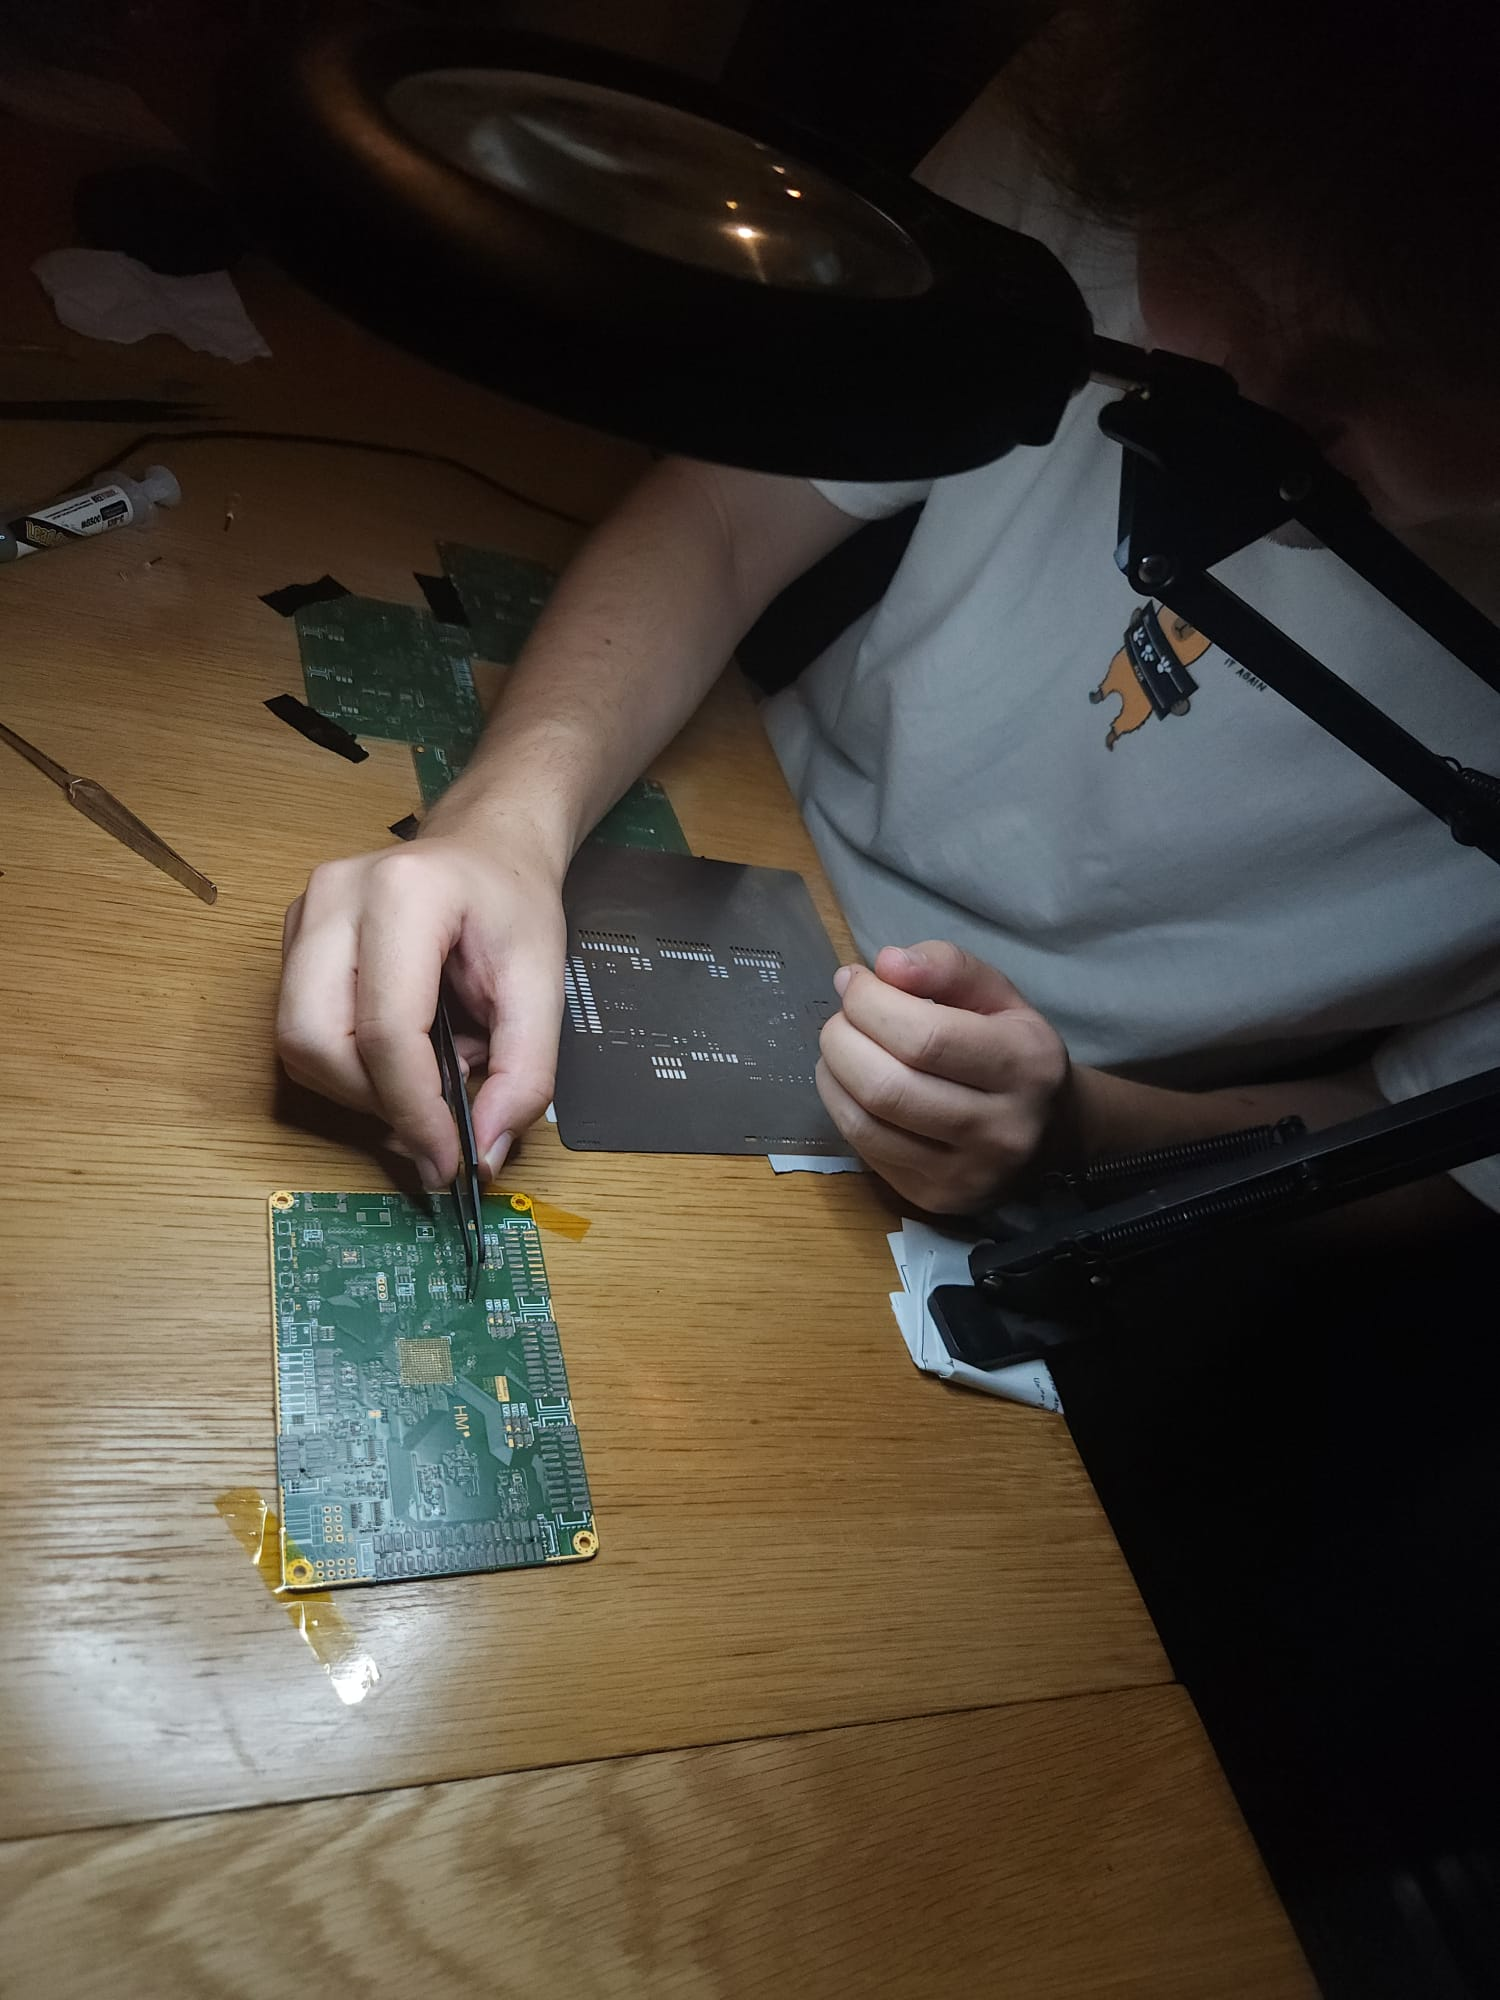
\includegraphics[width=0.7\textwidth]{assets/smd_bestueckung.jpg}
	\caption{Manuelle Platzierung der SMD-Komponenten mittels Pinzette}
	\label{fig:bestueckung}
\end{figure}

Der eigentliche Lötprozess erfolgte auf einer kompakten SMD-Heizplatte (Hotplate), die das PCB erhitzte, bis die Lotpaste aufschmolz und die Bauteile durch die Oberflächenspannung in Position zog. Da dieses manuelle Reflow-Verfahren weniger präzise steuerbar ist als ein industrieller Reflow-Ofen, kam es vereinzelt zu kleinen Fehlern wie Lötbrücken (Shorts) an eng benachbarten IC-Pins. Diese Fehlerstellen wurden nach einer gründlichen optischen Inspektion in einem manuellen Rework-Prozess mit einer feinen Lötspitze und Flussmittel behoben, bis alle Verbindungen fehlerfrei waren.

Trotz der manuellen Hürden konnten wir den Bestückungsprozess erfolgreich abschließen. Das fertig gelötete Board (siehe Abbildung~\ref{fig:pcb_fertig}) bildete schließlich die physische Grundlage für die darauffolgenden Bringup-Tests.

\begin{figure}[H]
	\centering
	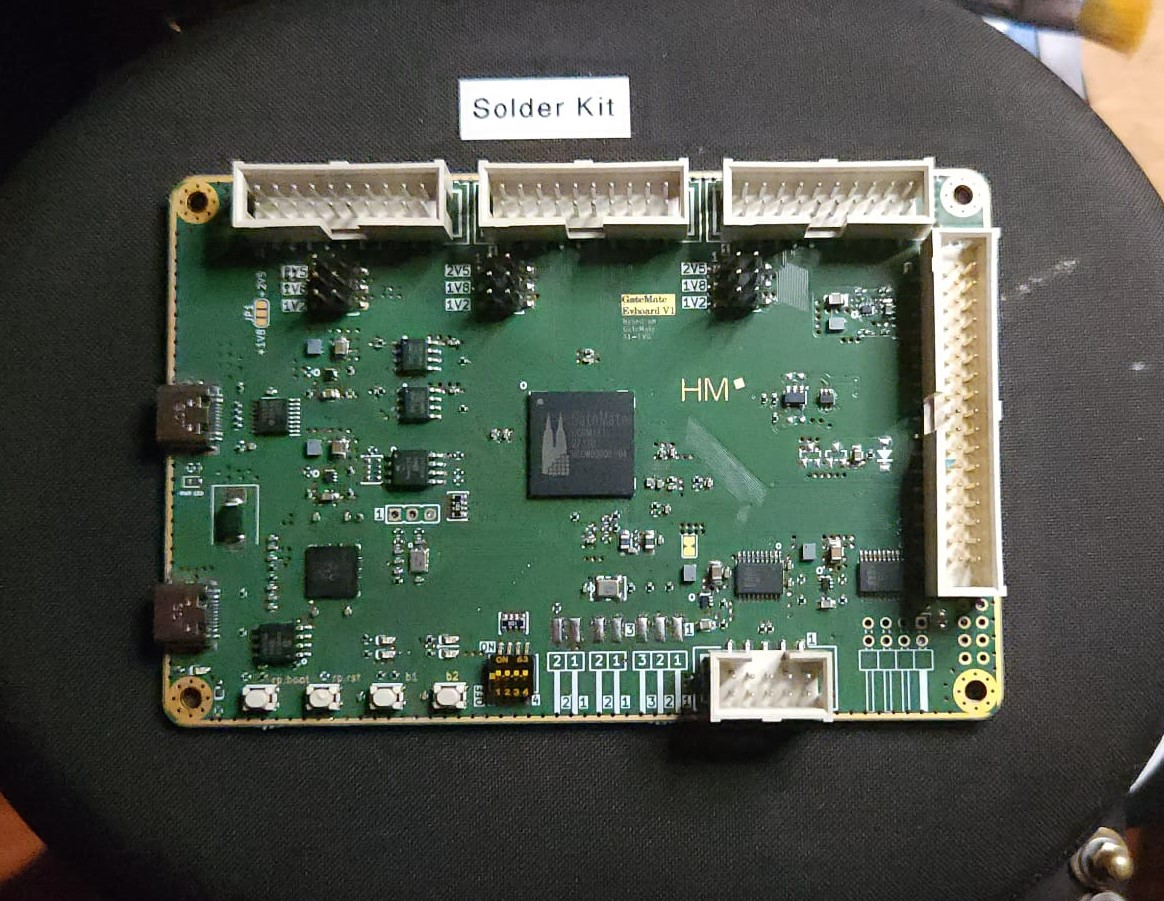
\includegraphics[width=0.8\textwidth]{assets/pcb_fertig.jpeg}
	\caption{Fertig bestückter und verlöteter Prototyp des GateMate Boards}
	\label{fig:pcb_fertig}
\end{figure}

\section{Bringup und Testinfrastruktur | Timo}

Nach dem erfolgreichen Abschluss der Bestückung und Lötung wurde der Hardware-Bringup schrittweise durchgeführt. Die Stufen 1 und 2 des Plans wurden dabei praktisch umgesetzt, während die weiteren Stufen als theoretische Vorbereitung für zukünftige Hardware-Revisionen dienen:
\begin{enumerate}
	\item \textbf{Stufe 1 – Power-Bringup (Smoke Test):} Vor der initialen Programmierung des FPGAs wurden alle Spannungsregler (LDOs, 3,3\,V, 1,8\,V Core-Voltage) ohne angeschlossene Peripherie mit einem Multimeter auf korrekte Pegel und Kurzschlüsse (Short-to-Ground) geprüft. Dieser Test verlief erfolgreich und verhinderte mögliche Hardware-Schäden beim anschließenden Betrieb.
	\item \textbf{Stufe 2 – Basis-Infrastruktur \& JTAG:} In dieser Stufe sollte der \texttt{10\,MHz} Oszillator mittels Oszilloskop auf ein sauberes Taktsignal geprüft werden. Dieser Test schlug jedoch fehl, da der entsprechende Oszillator bei der DigiKey-Bestellung leider untergegangen ist (als externes Element nicht direkt gelistet) und somit auf der Platine fehlte. Die detaillierte Fehlersuche und das Debugging dieser fehlenden Clock sind im Abschnitt von Fynn beschrieben, da er über die dafür nötige Messhardware verfügte.
	\item \textbf{Stufe 3 – USB-PHY Test (Geplant):} Aktivierung des TUSB1106. Es soll überprüft werden, ob der Host-PC die 1,5\,k$\Omega$ Full-Speed-Terminierung am D+-Pin korrekt erkennt. Mittels Oszilloskop werden die Signalpegel an den differentiellen Datenleitungen gemessen.
	\item \textbf{Stufe 4 – ISO/IEC-7816 Interface Test (Geplant):} Validierung des TXB0108-Levelshifters. Über Test-Pattern im FPGA wird geprüft, ob die Umschaltung der Power-Domains für die Smart Card (5\,V, 3\,V, 1,8\,V) lastfrei und sauber funktioniert, bevor echte Karten gesteckt werden.
\end{enumerate}
\newpage
\section{Ibex RISC-V Core und SV-Module | Xaver}

Der Ibex RISC-V Core ist ein Open-Source-32-Bit-RISC-V-Prozessor, der in SystemVerilog entwickelt wurde. Er eignet sich insbesondere für Embedded-Systeme und kann auf verschiedenen FPGA-Plattformen eingesetzt werden. Im folgenden Bild ist eine vereinfachte Darstellung der Architektur des Ibex zu sehen. Auf die einzelnen Komponenten und deren Zusammenspiel wird im Folgenden genauer eingegangen.

% HINWEIS: blockdiagram.pdf existiert nicht in ibex_bilder, deshalb auskommentiert
% \begin{figure}[H]
%     \centering
%     \includegraphics[width=0.8\textwidth]{ibex_bilder/blockdiagram.pdf}
%     \caption{Ibex Core Gesamtbild}
%     \label{fig:ibex_architektur_block}
% \end{figure}

\subsection{Instruction Memory und Data Memory}
Für das GateMate wurde ein Dual-Port-RAM mit einer Speichergröße von 4,KiB verwendet. Der RAM besitzt zwei voneinander unabhängige Ports. Port A wird für Zugriffe auf den Data Memory verwendet, während Port B für das Lesen von Instruktionen aus dem Instruction Memory zuständig ist.

Dies ist auch im SystemVerilog-Code der Instanz \texttt{ram\_2p} zu erkennen. Beim Port B ist \texttt{b\_we\_i} konstant auf \texttt{0} gesetzt. Dadurch kann über diesen Port ausschließlich gelesen und nicht geschrieben werden. Ebenso ist \texttt{b\_wdata\_i} konstant auf \texttt{0} gesetzt, da für einen reinen Lesezugriff keine Schreibdaten benötigt werden.

Ein wichtiger Unterschied besteht außerdem in der Anbindung an den Bus. Der Data Memory ist über Port A an den Bus angebunden. Dadurch können Schreib- und Lesezugriffe des Ibex über den Data-Port an den Bus weitergeleitet und anschließend an den RAM übertragen werden. Der Instruction Memory ist dagegen nicht an den Bus angebunden. Der Ibex greift über seinen separaten Instruction-Port direkt auf Port B des Dual-Port-RAMs zu. Dadurch sind Instruction Fetches und Datenzugriffe voneinander getrennt.

\subsection{Top Modul Demosystem}
% HINWEIS: ibex_top.svg kann von pdflatex nicht direkt kompiliert werden, deshalb auskommentiert
% \begin{figure}[H]
%     \centering
%     \includesvg[width=0.8\textwidth]{ibex_bilder/ibex_top.svg}
%     \caption{Vereinfachte Architektur des Top-Moduls}
%     \label{fig:ibex_architektur_top}
% \end{figure}
Schaut man sich das Top-Level des Demo-Systems an, das auf dem GateMate-FPGA eingesetzt wurde, lassen sich mehrere wichtige Komponenten erkennen, die im System instanziiert sind:

\begin{itemize}
	\item \texttt{ram\_2p}
	\item \texttt{ibex\_top}
	\item \texttt{bus}
	\item \texttt{gpio}
	\item \texttt{uart}
	\item \texttt{timer}
\end{itemize}

Einige Komponenten des ursprünglichen Demo-Systems wurden entfernt, um das System zu vereinfachen und an die begrenzten Ressourcen des GateMate-FPGAs anzupassen.

Eine zentrale Komponente des Systems ist der Bus. Dieser unterscheidet zwischen sogenannten \textit{Hosts} und \textit{Devices}. Ein Host ist dabei ein Modul, das Speicherzugriffe anfordert, während ein Device auf diese Zugriffe reagiert. In der aktuellen Konfiguration ist der Data-Port des Ibex der einzige Host. Als Devices sind unter anderem der RAM, das GPIO-, UART- und Timer-Modul angebunden. Aus diesem Grund besitzt die Bus-Schnittstelle sowohl \texttt{host\_*}- als auch \texttt{device\_*}-Signale.

Betrachten wir dazu einen konkreten Datenzugriff. Angenommen, im C-Code ist eine globale Variable definiert:

\begin{verbatim}
int a = 0x0F0F0F0F;

int main(void) {
return a;
}
\end{verbatim}

Für die Betrachtung des prinzipiellen Ablaufs werden Compileroptimierungen, der Startup-Code und weitere Vorgänge vor dem Aufruf von \texttt{main()} zunächst ignoriert.

Nehmen wir an, dass die globale Variable \texttt{a} entsprechend dem verwendeten Linkerskript an der Adresse \texttt{0x001004e0} liegt. Wenn die CPU in \texttt{main()} auf \texttt{a} zugreift, muss der Ibex den Wert aus dieser Speicheradresse lesen. Dazu erzeugt der Ibex über seinen Data-Port eine Anfrage mit der entsprechenden Adresse. Da es sich um einen Lesezugriff handelt, wird das Write-Signal deaktiviert.

Diese Anfrage wird im Top-Level über die \texttt{host\_*}-Signale an den Bus weitergeleitet. Dazu gehören unter anderem:

\begin{verbatim}
host_req
host_addr
host_we
host_be
host_wdata
\end{verbatim}

Der Bus überprüft anhand der Adresse, welchem Device der Zugriff zugeordnet werden muss. Dazu werden für jedes Device eine Basisadresse und eine Adressmaske definiert. Die Adresse \texttt{0x001004e0} liegt beispielsweise im Adressbereich des RAMs. Der Bus leitet die Anfrage deshalb über die entsprechenden \texttt{device\_*}-Signale an das RAM weiter.

Für das RAM sind dies unter anderem:

\begin{verbatim}
device_req[Ram]
device_addr[Ram]
device_we[Ram]
device_be[Ram]
device_wdata[Ram]
\end{verbatim}

Das RAM liefert den angeforderten Wert anschließend über \texttt{device\_rdata[Ram]} an den Bus zurück. Der Bus leitet diesen Wert über \texttt{host\_rdata[CoreD]} zurück an den Data-Port des Ibex. Die CPU erhält damit den Wert \texttt{0x0F0F0F0F} und kann ihn beispielsweise als Rückgabewert von \texttt{main()} verwenden.

Wichtig ist hierbei, dass \texttt{device\_rdata} kein Speicher und auch kein zweidimensionaler Speicherbereich ist. In SystemVerilog handelt es sich um ein Array von Signalen, wobei jedes Array-Element den Datenwert eines bestimmten Devices repräsentiert. Bei fünf Devices existieren beispielsweise \texttt{device\_rdata[0]} bis \texttt{device\_rdata[4]}. Diese Signale werden in der realen Hardware nicht als Software-Datenstruktur umgesetzt, sondern entsprechen Verbindungen zwischen den verschiedenen Schaltungskomponenten.

Der prinzipielle Datenfluss bei einem Lesezugriff auf die Variable \texttt{a} ist somit:
\newpage
\begin{verbatim}
Ibex Data-Port
|
| host_*
v
BUS
|
| device_* für Ram
v
ram_2p Port A
|
| device_rdata[Ram]
v
BUS
|
| host_rdata[CoreD]
v
Ibex Data-Port
\end{verbatim}

Der Instruction Memory stellt dabei einen Sonderfall dar: Instruction Fetches des Ibex laufen nicht über den Bus, sondern über den zweiten Port des Dual-Port-RAMs direkt zum RAM. Der Bus ist somit für die Datenzugriffe des Ibex zuständig, während der Instruction Fetch einen separaten Pfad verwendet.

\subsection{Register File}
Das Register File des Ibex Prozessors enthält je nach Konfiguration entweder 32 oder 16 Register.
Wird der Parameter \texttt{RV32E} deaktiviert, stehen die Register \texttt{x0} bis \texttt{x31} zur Verfügung.
Da das Register \texttt{x0} bei der RISC-V Architektur jedoch konstant den Wert 0 liefert und nicht beschrieben werden darf, müssen tatsächlich nur 31 Register gespeichert werden.
Bei aktivierter \texttt{RV32E}-Erweiterung reduziert sich das Register File auf die Register \texttt{x0} bis \texttt{x15}, wodurch nur 15 Register gespeichert werden müssen.

Die Register werden im SystemVerilog als zweidimensionales Array dargestellt:

\begin{verbatim}
logic [DataWidth-1:0] mem[NUM_WORDS];
\end{verbatim}

Dabei entspricht jedes Element des Arrays einem 32-Bit breiten Register.

Für die Implementierung auf dem GateMate FPGA wird die Datei
\texttt{ibex\_register\_file\_fpga.sv} verwendet. Diese Implementierung ist so geschrieben, dass Synthesetools das Register File möglichst effizient auf die vorhandenen FPGA-Ressourcen abbilden können. Je nach FPGA-Architektur und Synthesetool kann das Register File beispielsweise durch Block RAMs oder durch Logikzellen (LUTs und Flip-Flops) implementiert werden.

Eine weitere Variante ist das \texttt{ibex\_register\_file\_ff.sv}.
Hier wird jedes einzelne Bit der Register durch ein Flip-Flop gespeichert.
Bei 32 Registern mit jeweils 32 Bit würde dies theoretisch 1024 einzelne Flip-Flops benötigen (das Register x0 wird hierbei nicht als normales Register gespeichert).

Die dritte Variante ist das \texttt{ibex\_register\_file\_latch.sv}.
Diese Implementierung basiert auf Latches und verwendet zusätzlich Clock-Gating, um den Energieverbrauch zu reduzieren.
Dabei wird nicht jedes Register bei jedem Takt aktiviert, sondern nur das Register, in welches aktuell geschrieben werden soll.
Hierfür wird zunächst anhand der Schreibadresse ein One-Hot-Signal erzeugt, welches anschließend die jeweilige Clock-Gating-Zelle aktiviert.

Dies ist im SystemVerilog-Code zu erkennen:

\begin{verbatim}
for (genvar x = 1; x < NUM_WORDS; x++) begin : gen_cg_word_iter
  prim_clock_gating cg_i (
      .clk_i     ( clk_int           ),
      .en_i      ( waddr_onehot_a[x] ),
      .test_en_i ( test_en_i         ),
      .clk_o     ( mem_clocks[x]     )
  );
end
\end{verbatim}

Wird beispielsweise in das Register \texttt{x5} geschrieben, wird nur die Clock für dieses Register aktiviert.
Das entsprechende Latch kann anschließend den neuen Wert übernehmen:

\begin{verbatim}
for (genvar i = 1; i < NUM_WORDS; i++) begin : g_rf_latches
  always_latch begin
    if (mem_clocks[i]) begin
      mem[i] = wdata_a_q;
    end
  end
end
\end{verbatim}

Diese Latch-basierte Variante ist hauptsächlich für ASIC-Implementierungen vorgesehen, da dort spezielle Clock-Gating-Zellen verfügbar sind. Für FPGAs wie den GateMate ist diese Implementierung ungeeignet und kann zu Syntheseproblemen führen. Deshalb wird für die FPGA-Implementierung die Variante \texttt{ibex\_register\_file\_fpga.sv} verwendet.

\subsection{Instruction Decode und Execute Stage}
Die \textbf{Instruction Decode and Execute Stage} übernimmt die vom Instruction-Fetch bereitgestellten Maschinenbefehle. Wurde zuvor eine komprimierte RISC-V-Instruktion (RVC) geladen, wird diese zunächst in ihre unkomprimierte Darstellung umgewandelt. Anschließend werden die Instruktionen innerhalb eines Taktzyklus dekodiert und ausgeführt. Dabei erfolgen auch das Lesen und Schreiben des Register Files.

Die zentrale Komponente dieser Stufe ist die \texttt{ibex\_id\_stage.sv}. Sie steuert den gesamten Dekodier- und Ausführungsprozess. Multiplexer wählen dabei die Operanden für die ALU sowie die Quelle der Daten aus, die in das Register File zurückgeschrieben werden. Für mehrzyklische Instruktionen besitzt die ID-Stage eine kleine Zustandsmaschine, welche die Pipeline während der Ausführung anhält.

Der \textbf{Controller} (\texttt{ibex\_controller.sv}) enthält die Hauptzustandsmaschine des Prozessors. Zu seinen Aufgaben gehören das Starten des Prozessors nach einem Reset, das Aktualisieren des Programmzählers bei Sprüngen und Verzweigungen, die Behandlung von Exceptions und Interrupts einschließlich der Aktualisierung der CSR-Register, die Steuerung des Schlafmodus (WFI) sowie die Unterstützung der Debug-Funktionalität.

Der \textbf{Decoder} (\texttt{ibex\_decoder.sv}) dekodiert die Maschinenbefehle und erzeugt die entsprechenden Steuersignale für die übrigen Komponenten der CPU. Anhand des Opcodes und weiterer Befehlsfelder wird bestimmt, welche Operation ausgeführt werden soll und welche Funktionsblöcke, wie beispielsweise die ALU oder das Register File, angesteuert werden.

\subsection{Toolchain | Xaver}
\subsubsection{FPGA Toolchain}
\begin{figure}[H]
	\centering
	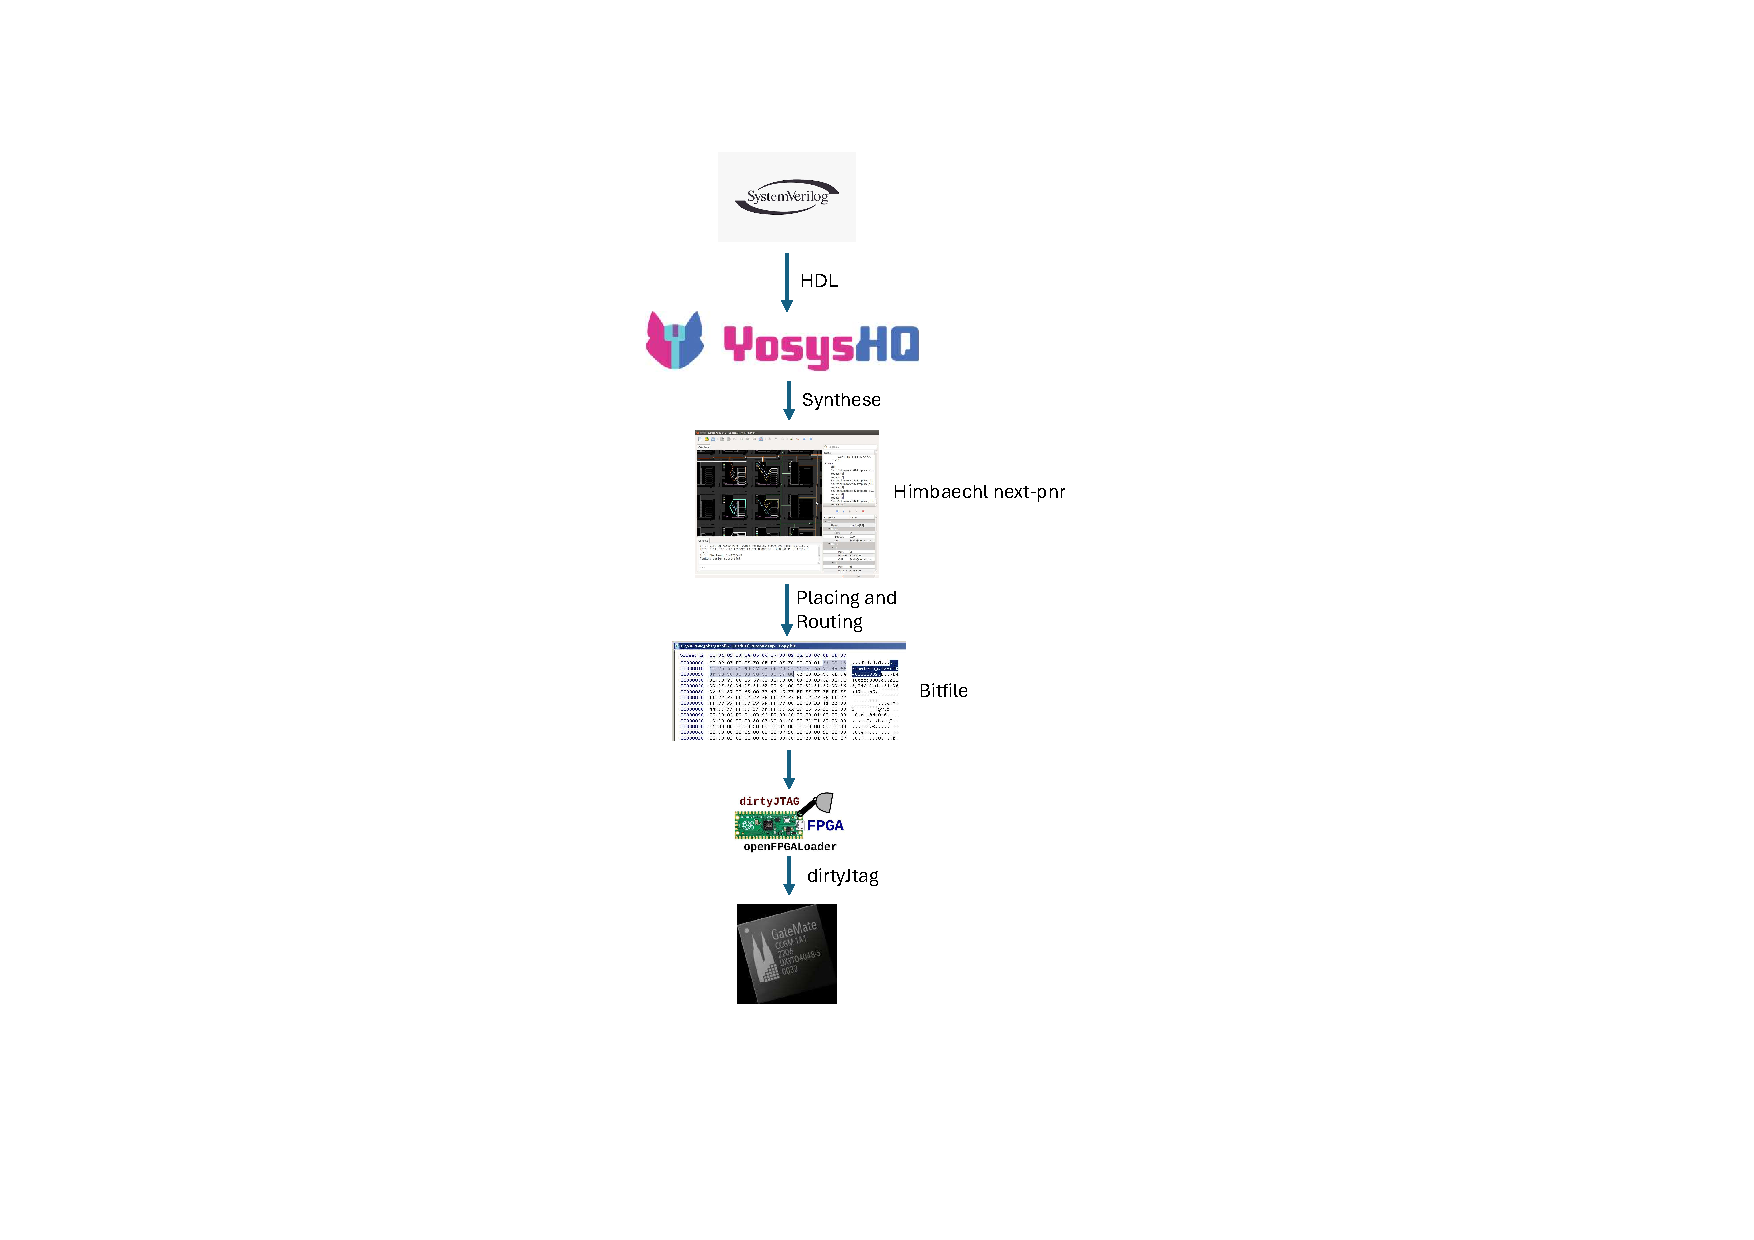
\includegraphics[width=1.0\textwidth,trim=5cm 3cm 2cm 1cm,clip]{ibex_bilder/toolchain_final.pdf}
	\caption{Toolchain Ablauf}
	\label{fig:toolchain_final}
\end{figure}


Um den Ibex-Prozessor auf dem GateMate FPGA ausführen zu können, musste zunächst eine vollständige Entwicklungsumgebung eingerichtet werden. Hierzu wurde die Open-Source-Toolchain der \textit{OSS CAD Suite} installiert. Diese enthält unter anderem die Werkzeuge \texttt{Yosys} zur Synthese sowie \texttt{nextpnr-himbaechel} für das Place-and-Route des GateMate FPGAs.

Anschließend wurde das Ibex-Repository geklont und das vorhandene Demo-System analysiert. Da das ursprüngliche Projekt auf ein anderes FPGA-Board ausgelegt war, mussten verschiedene Anpassungen vorgenommen werden, um eine lauffähige GateMate-Version zu erhalten. Hierzu gehörten insbesondere die Anpassung der Taktfrequenz, der Speichergröße sowie das Entfernen nicht benötigter Peripherie, um die Routing-Auslastung des FPGAs zu reduzieren.

Für die Erzeugung der FPGA-Konfiguration wurde ein eigenes \texttt{Makefile} erstellt. Dieses automatisiert den gesamten Build-Prozess und führt die einzelnen Werkzeuge der Toolchain nacheinander aus. Der Ablauf umfasst die Synthese des SystemVerilog-Codes mit \texttt{Yosys}, das Place-and-Route mit \texttt{nextpnr-himbaechel} sowie die Erzeugung des GateMate-Bitstreams.

Zur Programmierung des GateMate FPGA wurde anschließend \texttt{openFPGALoader} zusammen mit einem DirtyJTAG-Adapter verwendet. Dadurch konnte der erzeugte Bitstream direkt über die JTAG-Schnittstelle auf das FPGA übertragen werden.

Neben der FPGA-Toolchain wurde ebenfalls eine RISC-V-Compiler-Toolchain eingerichtet. Diese dient zur Übersetzung von C-Programmen in RISC-V-Maschinencode. Anschließend werden die erzeugten ELF- und Binärdateien in den Initialisierungsspeicher des Demo-Systems eingebunden, sodass der Prozessor das Programm nach dem Konfigurieren des FPGA direkt ausführen kann.

Nach erfolgreicher Einrichtung der Entwicklungsumgebung konnte der komplette Entwicklungsablauf automatisiert werden. Dieser umfasst das Kompilieren der Software, die Synthese der Hardware, das Place-and-Route, die Bitstream-Erzeugung sowie das Programmieren des GateMate FPGA.

\subsection{C Code Generierung}
\begin{figure}[H]
	\centering
	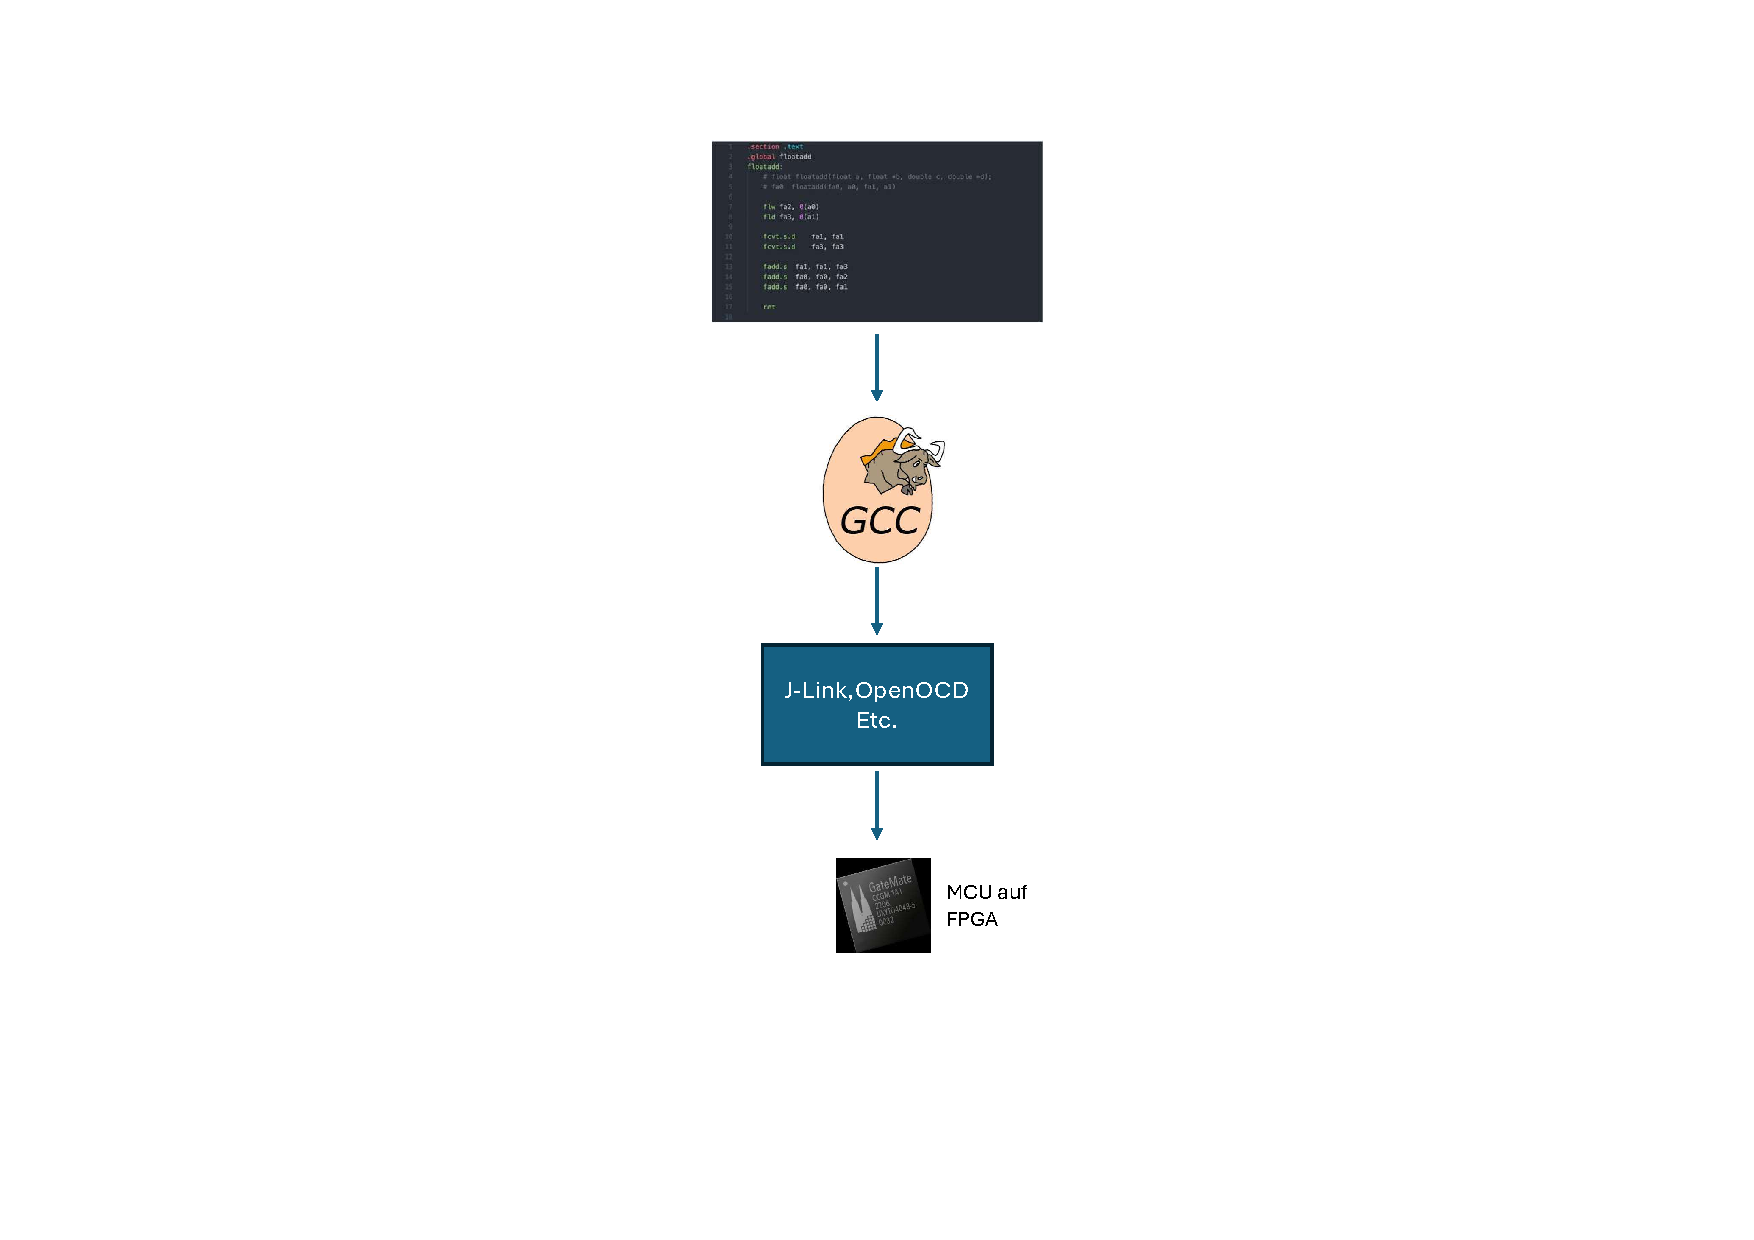
\includegraphics[width=1.0\textwidth,trim=7cm 4cm 2cm 1cm,clip]{ibex_bilder/normal_compile.pdf}
	\caption{Häufigster Flash Vorgang}
	\label{fig:normal_compile}
\end{figure}

Bei klassischen Mikrocontrollern wird die Firmware üblicherweise zunächst mit einem Compiler aus dem C-Quellcode in Maschinencode übersetzt. Anschließend erzeugt der Linker eine ausführbare Datei, welche die Speicheradressen der einzelnen Programmteile festlegt. Aus dieser Datei wird häufig eine Binär- oder HEX-Datei erzeugt, welche anschließend in den Flash-Speicher des Mikrocontrollers programmiert wird.

Der Flash-Vorgang erfolgt abhängig von der verwendeten Mikrocontroller-Plattform über verschiedene Schnittstellen. Häufig verwendete Verfahren sind beispielsweise:

\begin{itemize}
	\item \textbf{SWD (Serial Wire Debug):} Wird hauptsächlich bei ARM Cortex-M Mikrocontrollern verwendet und ermöglicht das Programmieren und Debuggen über wenige Pins.
	\item \textbf{JTAG:} Eine weit verbreitete Debug- und Programmierschnittstelle, die insbesondere bei komplexeren Mikrocontrollern und Prozessoren eingesetzt wird.
	\item \textbf{Bootloader-basierte Programmierung:} Viele Mikrocontroller besitzen einen integrierten Bootloader, über den die Firmware beispielsweise über UART, USB oder CAN übertragen werden kann.
	\item \textbf{Herstellerspezifische Programmer:} Beispiele hierfür sind ST-Link für STM32-Mikrocontroller oder ähnliche Programmieradapter anderer Hersteller.
\end{itemize}

Der typische Ablauf besteht somit aus:
\begin{center}
	C-Quellcode $\rightarrow$ Compiler $\rightarrow$ ELF-Datei $\rightarrow$ BIN/HEX-Datei $\rightarrow$ Programmer $\rightarrow$ Flash-Speicher der MCU
\end{center}

Im Gegensatz zu einem klassischen Mikrocontroller besitzt der verwendete Ibex-Prozessor auf dem GateMate FPGA keinen internen Flash-Speicher für die Firmware. Daher wird die Software nicht nachträglich über eine Programmierschnittstelle in einen Speicher geschrieben. Stattdessen wird das Programm bereits während der FPGA-Erstellung in den Instruction Memory integriert.

Hierzu wird der erzeugte RISC-V-Maschinencode als Initialinhalt des RAMs eingebunden. Der Instruction Memory wird somit bereits im SystemVerilog-Code mit den entsprechenden Instruktionen initialisiert. Während der Synthese wird dieser Speicherinhalt zusammen mit der Hardwarebeschreibung verarbeitet und anschließend im FPGA-Bitstream gespeichert.

Der Ablauf unterscheidet sich somit von einer klassischen MCU-Programmierung:

\begin{center}
	C-Quellcode $\rightarrow$ RISC-V Compiler $\rightarrow$ Speicherinitialisierung $\rightarrow$ SystemVerilog Synthese $\rightarrow$ FPGA Bitstream $\rightarrow$ Instruction Memory
\end{center}

Nach der Konfiguration des GateMate FPGAs steht der Programmcode dem Ibex-Core direkt im Instruction Memory zur Verfügung und kann ohne separaten Flash-Vorgang ausgeführt werden.

\section{Ablauf, Probleme und Erfolge | Xaver}
\subsection{Ablauf}

Um den Ibex auf dem Olimex GateMate A1 zu portieren, wurde zunächst mit einfachen Blinky-Programmen begonnen. Das Ziel dieser ersten Schritte bestand darin, sich mit dem FPGA-Board sowie der benötigten Toolchain vertraut zu machen und den grundlegenden Entwicklungs- und Programmierablauf zu überprüfen.

Die Installation der benötigten Toolchain kann unkompliziert über die OSS CAD Suite erfolgen. Diese stellt unter anderem die für die Synthese sowie für die anschließende Implementierung benötigten Open-Source-Werkzeuge bereit. Die aktuelle Version ist unter \verb|https://github.com/YosysHQ/oss-cad-suite-build/releases| verfügbar. Für die Verwendung der Toolchain wird ein Linux-Betriebssystem empfohlen, da die verwendeten Werkzeuge dort direkt und ohne zusätzliche Kompatibilitätsschichten eingesetzt werden können.

Nach den ersten erfolgreichen Implementierungen wurde ein \texttt{Makefile} eingeführt, um die einzelnen Schritte des FPGA-Entwicklungsprozesses zu automatisieren. Das finale Makefile sieht wie folgt aus:

\begin{verbatim}
TOP = top_gatemate

# You can deactivate the seed, it is not necessary
PREFIX := rtl/
DESIGN_SOURCES := $(addprefix $(PREFIX),$(shell cat build/compile_files.txt))

IMPLEMENT_FLAGS = -l Logs/routing.log --verbose --device=CCGM1A1 \
                  --seed 1 --vopt allow-unconstrained \
                  --json Synth/$(TOP)_synth_final.json

GATE_MATE_PIN_CONSTRAINTS = constraints/pin_constraints.ccf
GATE_MATE_TIMING_CONSTRAINTS = constraints/timing_constraints.sdc

soc:
	# Synthesize with Yosys. The slang plugin is required
	# for modern SystemVerilog syntax.
	yosys -m slang -p "read_slang --std latest \
	--ignore-initial $(DESIGN_SOURCES) --top $(TOP) \
	-D SYNTHESIS; synth_gatemate -top $(TOP) -luttree \
	-nomx8; write_verilog Synth/$(TOP)_synth.v; \
	write_json Synth/$(TOP)_synth_final.json" > Logs/synth.log

	# Implement (place and route) with nextpnr.
	nextpnr-himbaechel $(IMPLEMENT_FLAGS) \
	-o ccf=$(GATE_MATE_PIN_CONSTRAINTS) \
	-o out=Impl/impl.txt \
	--sdc $(GATE_MATE_TIMING_CONSTRAINTS) \
	--router router2

	# Create bitfile with gmpack.
	gmpack Impl/impl.txt Impl/impl.bit

clean:
	rm -f *.log *.png Synth/*.v Synth/*.json \
	Impl/*.bit Impl/*.txt Logs/*.log
\end{verbatim}

Das Makefile automatisiert damit die vollständige Erstellung des FPGA-Bitstreams. Der Prozess lässt sich grundsätzlich in drei Schritte unterteilen: Synthese, Place-and-Route sowie die Erzeugung des finalen Bitfiles.

Im ersten Schritt wird mit \texttt{Yosys} die Synthese des Designs durchgeführt. Hierbei werden die angegebenen SystemVerilog-Quelldateien eingelesen und in eine für das GateMate-FPGA geeignete Netzliste überführt. Für die Verarbeitung moderner SystemVerilog-Syntax wird das \texttt{slang}-Plugin verwendet. Zusätzlich wird mit \texttt{synth\_gatemate} eine für die GateMate-Architektur angepasste Synthese durchgeführt. Als Ergebnis werden unter anderem eine JSON-Datei sowie eine synthetisierte Verilog-Datei erzeugt. Die JSON-Datei dient anschließend als Eingabe für den Place-and-Route-Schritt.

Im zweiten Schritt übernimmt \texttt{nextpnr-himbaechel} die Implementierung des Designs. Dabei werden die logischen Ressourcen des Designs auf die physikalischen Ressourcen des GateMate-FPGAs abgebildet (Placement) und anschließend die notwendigen Verbindungen zwischen diesen Ressourcen hergestellt (Routing).

Zusätzlich werden zwei Constraint-Dateien übergeben. Die \texttt{CCF}-Datei (\textit{Calypto Constraint Format}) definiert insbesondere die Zuordnung der Design-Signale zu den physischen I/O-Pins des FPGAs. Dadurch wird beispielsweise festgelegt, an welchem Pin des FPGA ein LED-Signal oder ein Taktsignal angeschlossen ist. Die \texttt{SDC}-Datei (\textit{Synopsys Design Constraints}) enthält hingegen Timing-Anforderungen des Designs, beispielsweise Vorgaben für verwendete Taktsignale.

Nach erfolgreichem Place-and-Route wird im letzten Schritt mit \texttt{gmpack} aus der erzeugten Implementierungsdatei das für den GateMate-FPGA benötigte Bitfile erzeugt:

\begin{verbatim}
gmpack Impl/impl.txt Impl/impl.bit
\end{verbatim}

Das erzeugte Bitfile kann anschließend auf das FPGA übertragen werden. Hierfür wird \texttt{DirtyJTAG} verwendet. Das Olimex GateMate A1-Board verfügt über einen integrierten Raspberry Pi, auf dem die für DirtyJTAG benötigte Software ausgeführt werden kann. Dadurch kann das FPGA direkt über die vorhandene Hardware-Schnittstelle programmiert werden.

Der gesamte Ablauf lässt sich somit wie folgt zusammenfassen:
\newpage
\begin{enumerate}
	\item Einlesen und Synthese des SystemVerilog-Designs mit Yosys.
	\item Erzeugung der GateMate-Netzliste.
	\item Placement und Routing mit nextpnr-himbaechel.
	\item Anwendung der Pin- und Timing-Constraints.
	\item Erzeugung des Bitfiles mit gmpack.
	\item Übertragung des Bitfiles auf das GateMate-FPGA mittels DirtyJTAG.
\end{enumerate}

\subsection{Probleme}

Eines der größten Probleme bei der Implementierung des Systems auf dem GateMate FPGA stellte die fehlende direkte Unterstützung von Clock Gating dar. Beim Clock Gating wird das Taktsignal abhängig von einem Enable-Signal aktiviert oder deaktiviert. Dadurch können beispielsweise ganze Teile eines Systems gezielt angehalten werden, wenn sie nicht benötigt werden.

In der verwendeten Implementierung wird das Taktsignal zunächst mit einer Logik verknüpft. Aus Sicht des Synthese- und Place-and-Route-Tools handelt es sich bei dem daraus resultierenden Signal jedoch nicht mehr um ein reguläres Taktsignal, sondern um ein gewöhnliches Logiksignal. Dadurch wird das Signal nicht mehr über die dedizierte Clock-Verteilung des FPGAs (Clock Tree) geführt. Dies kann insbesondere bei größeren Schaltungen zu Problemen hinsichtlich der Taktverteilung und der Laufzeitunterschiede des Taktsignals (Clock Skew) führen.

Grundsätzlich lässt sich dieses Problem durch die Verwendung spezieller FPGA-spezifischer Primitives lösen, die eine geeignete Taktgatterung und deren Einbindung in die Clock-Struktur des FPGAs ermöglichen. Eine solche Lösung wurde im Rahmen dieses Projekts jedoch nicht umgesetzt. Stattdessen wurde die Clock-Gating-Funktionalität für die verwendete Implementierung entsprechend angepasst.

\begin{figure}[H]
	\centering
	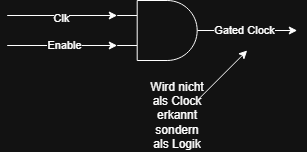
\includegraphics[width=0.7\textwidth]{ibex_bilder/gated_clock2.png}
	\caption{Prinzip eines gated Clock-Signals}
	\label{fig:gated_clock}
\end{figure}

\subsection{Erfolge}

Zu den wesentlichen Erfolgen des Projekts zählt die erfolgreiche Inbetriebnahme des Ibex-Prozessors auf dem Olimex-Board mit dem darauf verwendeten GateMate FPGA. Hierfür wurde zunächst die bestehende Ibex-Implementierung analysiert und an die vorhandene Hardware sowie die Anforderungen des Projekts angepasst. Dabei wurden unter anderem nicht benötigte Komponenten des ursprünglichen Systems entfernt und die Speicher- und Peripheriekonfiguration entsprechend angepasst.

Ein weiterer wichtiger Erfolg war die erfolgreiche Implementierung und Anbindung einer UART-Schnittstelle. Dadurch war es möglich, Daten direkt vom auf dem FPGA ausgeführten Ibex-Prozessor an ein Terminal auf dem PC zu übertragen und die Funktion des Prozessors sowie der implementierten Peripherie praktisch zu überprüfen. Im Verlauf der Entwicklung wurde die UART-Schnittstelle schrittweise erweitert und an die Anforderungen des Systems angepasst.

Zusätzlich wurde ein eigenes Baudratenregister implementiert. Dadurch kann die Baudrate der UART-Schnittstelle über ein Register konfiguriert werden, anstatt diese ausschließlich zur Compile-Zeit fest vorzugeben. Dies stellt eine Erweiterung der ursprünglichen Peripheriefunktionalität dar und ermöglicht eine flexiblere Verwendung der UART-Schnittstelle.

Im Rahmen der Implementierung wurden außerdem verschiedene Anpassungen an der Hardwarebeschreibung und der Software vorgenommen, um das Zusammenspiel zwischen Prozessor, Speicher und Peripherie sicherzustellen. Hierzu gehörten unter anderem die Anpassung der Adressbereiche, die Integration der zusätzlichen Register sowie die Erstellung und Anpassung der benötigten Software für die Kommunikation mit den Peripheriekomponenten.

Insgesamt konnte damit eine funktionsfähige Grundlage geschaffen werden, auf der der Ibex-Prozessor eigenständig auf dem GateMate FPGA ausgeführt wird und über die implementierte UART-Schnittstelle mit einem externen System kommunizieren kann.

\section{Nutzung von KI}
Im Rahmen des Projekts wurden KI-Tools unterstützend eingesetzt, insbesondere zur Recherche, zur Fehlersuche (Debugging) sowie zur sprachlichen Überarbeitung und Formatierung der Dokumentation. Die grundlegenden Design-Entscheidungen, die Architektur der Schaltung sowie die technische Umsetzung wurden eigenständig vom Team erarbeitet; KI-Tools dienten dabei lediglich als Hilfsmittel zur Effizienzsteigerung und Qualitätssicherung, nicht als Quelle der eigentlichen Projektinhalte.

\section{Verwendete Bilder}
Jedliche in dieser Arbeit verwendete Grafik wurde von den Autoren erstellt und ist unter keinem Copyright.

\section{Quellcode}
Alle Hardware und Software Dokumente sind unter \href{https://github.com/Flynsky/MillerProject}{https://github.com/Flynsky/MillerProject} abrufbar.

\section{Schematic}
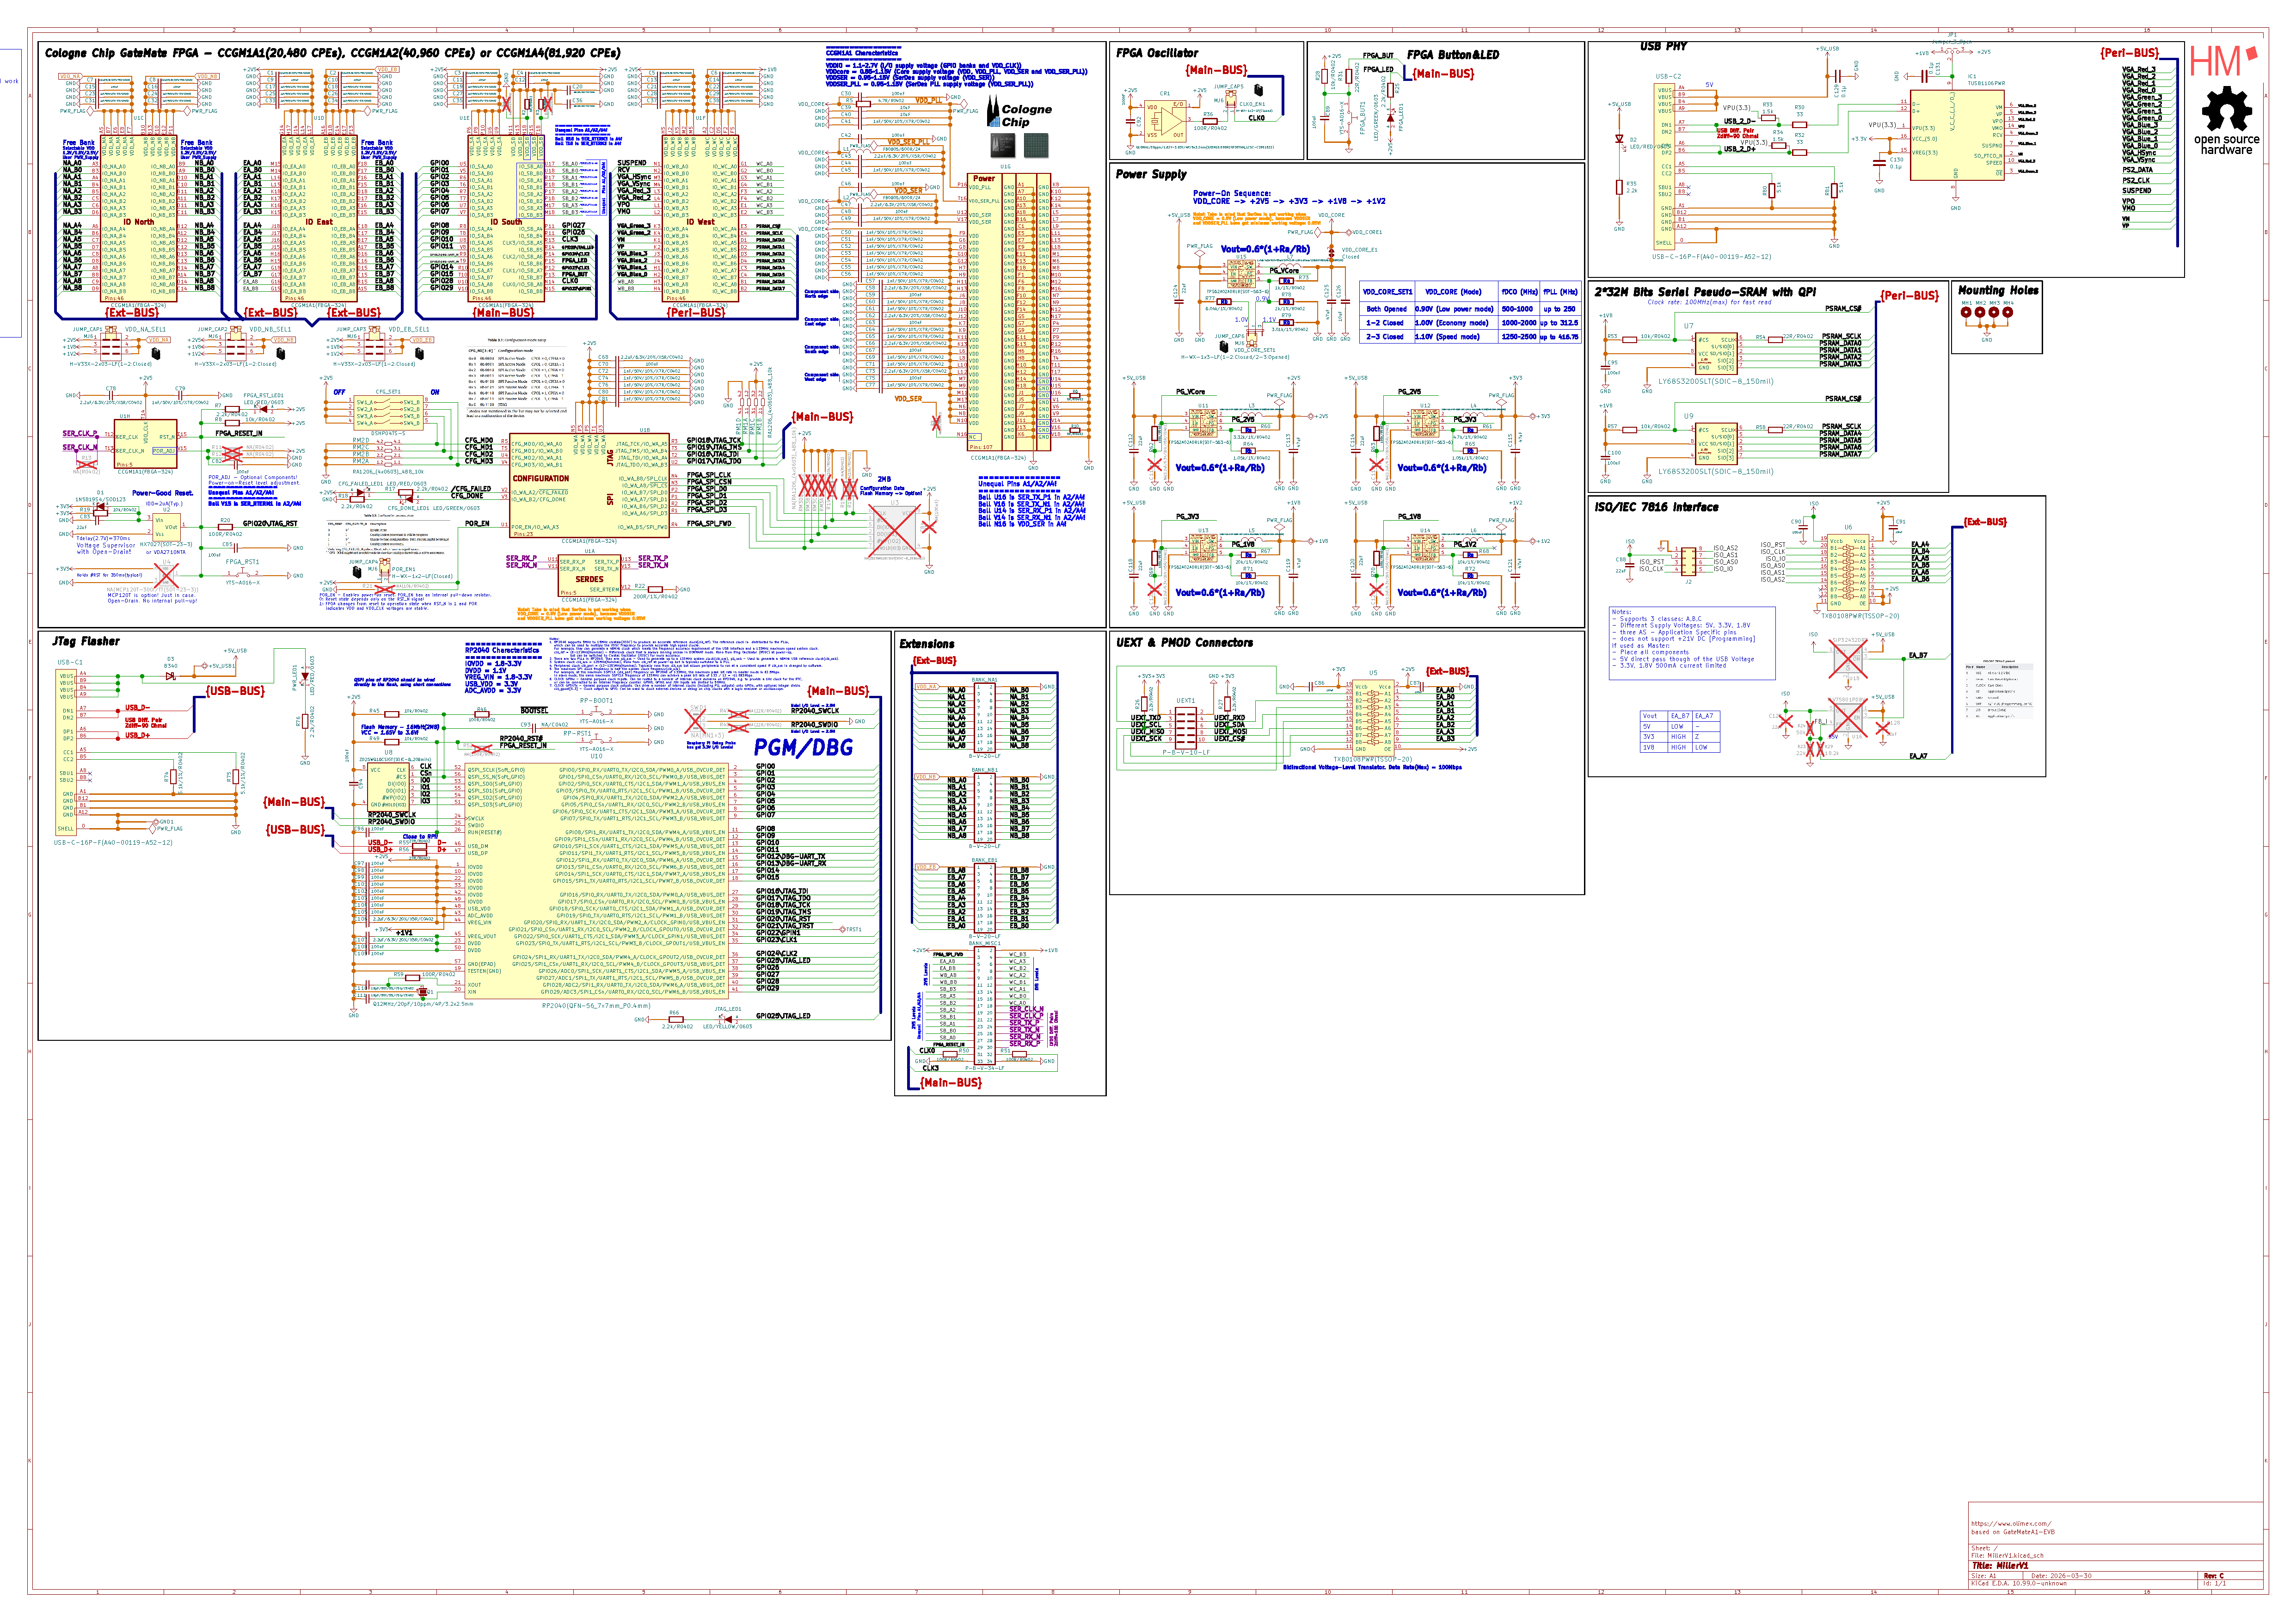
\includepdf[pages=-, angle=90]{../../hardware/MillerV1/MillerV1.pdf}

\end{document}
